\documentclass{article}
\title{Mathematics for Machine Learning}
\author{Garrett Thomas\\
Department of Electrical Engineering and Computer Sciences\\
University of California, Berkeley}

% useful packages
\usepackage{amsfonts,amsmath,amssymb,amsthm,bm,commath,enumerate,graphicx,hyperref,nicefrac,physics,subcaption}

% formatting
\setlength{\parskip}{0.5em}
\setlength{\parindent}{0em}
\usepackage[margin=1.25in]{geometry}
\hypersetup{
    colorlinks=true,
    linktoc=all,
    linkcolor=black,
    urlcolor=blue
}

% shorthand
\DeclareMathOperator*{\argmax}{arg\,max}
\DeclareMathOperator*{\argmin}{arg\,min}
\DeclareMathOperator*{\dom}{dom}
\DeclareMathOperator*{\range}{range}
\DeclareMathOperator*{\diag}{diag}
\newcommand{\C}{\mathbb{C}}
\newcommand{\F}{\mathbb{F}}
\newcommand{\N}{\mathbb{N}}
\newcommand{\Q}{\mathbb{Q}}
\newcommand{\R}{\mathbb{R}}
\newcommand{\Z}{\mathbb{Z}}
\newcommand{\calA}{\mathcal{A}}
\newcommand{\calB}{\mathcal{B}}
\newcommand{\calC}{\mathcal{C}}
\newcommand{\calD}{\mathcal{D}}
\newcommand{\calF}{\mathcal{F}}
\newcommand{\calH}{\mathcal{H}}
\newcommand{\calI}{\mathcal{I}}
\newcommand{\calL}{\mathcal{L}}
\newcommand{\calM}{\mathcal{M}}
\newcommand{\calN}{\mathcal{N}}
\newcommand{\calP}{\mathcal{P}}
\newcommand{\calR}{\mathcal{R}}
\newcommand{\calX}{\mathcal{X}}
\renewcommand{\vec}[1]{\mathbf{#1}}
\newcommand{\mat}[1]{\mathbf{#1}}
\newcommand{\matlit}[1]{\begin{bmatrix}#1\end{bmatrix}}
\newcommand{\tran}{^\top}
\newcommand{\inv}{^{-1}}
\newcommand{\halfpow}{^{\frac{1}{2}}}
\newcommand{\neghalfpow}{^{-\frac{1}{2}}}
\renewcommand{\angle}[1]{\langle #1 \rangle}
\newcommand{\inner}[2]{\angle{#1, #2}}
\renewcommand{\P}{\mathbb{P}}
\newcommand{\pr}[1]{\P(#1)}
\newcommand{\prbig}[1]{\P\big(#1\big)}
\newcommand{\prbigg}[1]{\P\bigg(#1\bigg)}
\newcommand{\prlr}[1]{\P\left(#1\right)}
\newcommand{\comp}{^\text{c}}
\newcommand{\given}{|}
\renewcommand{\ev}[1]{\mathbb{E}[#1]}
\newcommand{\evwrt}[2]{\mathbb{E}_{#1}[#2]}
\renewcommand{\var}[1]{\operatorname{Var}(#1)}
\newcommand{\cov}[2]{\operatorname{Cov}(#1, #2)}
\newcommand{\bigev}[1]{\mathbb{E}\left[#1\right]}
\newcommand{\bigvar}[1]{\operatorname{Var}\left(#1\right)}
\newcommand{\bigcov}[2]{\operatorname{Cov}\left(#1, #2\right)}
\newcommand{\iid}{\overset{\text{iid}}{\sim}}
\newcommand{\bX}{\mathbf{X}}
\newcommand{\term}[1]{\textbf{#1}}
\newcommand{\tab}{\hspace{0.5cm}}
\renewcommand{\a}{\vec{a}}
\renewcommand{\b}{\vec{b}}
\newcommand{\g}{\vec{g}}
\newcommand{\h}{\vec{h}}
\renewcommand{\o}{\vec{o}}
\newcommand{\q}{\vec{q}}
\newcommand{\s}{\vec{s}}
\newcommand{\x}{\vec{x}}
\newcommand{\y}{\vec{y}}
\newcommand{\w}{\vec{w}}
\newcommand{\z}{\vec{z}}
\newcommand{\A}{\mat{A}}
\newcommand{\I}{\mat{I}}
\newcommand{\xye}{\tilde{\x}}
\newcommand{\dotcup}{\mathbin{\dot{\cup}}}
\newcommand{\bigdotcup}{\mathop{\dot{\bigcup}}}

\newtheorem{theorem}{Theorem}
\newtheorem*{theorem*}{Theorem}
\newtheorem{definition}{Definition}
\newtheorem*{definition*}{Definition}
\newtheorem{proposition}{Proposition}
\newtheorem*{proposition*}{Proposition}
\newtheorem{lemma}{Lemma}
\newtheorem*{lemma*}{Lemma}
\newtheorem{corollary}{Corollary}
\newtheorem*{corollary*}{Corollary}
\theoremstyle{remark}
\newtheorem*{note}{Note}
\newtheorem*{example}{Example}


\begin{document}
\maketitle

\section{About}
Machine learning uses tools from a variety of mathematical fields.
This document is an attempt to provide a summary of the mathematical background needed for an introductory class in machine learning, which at UC Berkeley is known as CS 189/289A.

Our assumption is that the reader is already familiar with the basic concepts of multivariable calculus and linear algebra (at the level of UCB Math 53/54).
We emphasize that this document is \textbf{not} a replacement for the prerequisite classes.
Most subjects presented here are covered rather minimally; we intend to give an overview and point the interested reader to more comprehensive treatments for further details.

Note that this document concerns math background for machine learning, not machine learning itself.
We will not discuss specific machine learning models or algorithms except possibly in passing to highlight the relevance of a mathematical concept.

Earlier versions of this document did not include proofs.
We have begun adding in proofs where they are reasonably short and aid in understanding.
These proofs are not necessary background for CS 189 but can be used to deepen the reader's understanding.

You are free to distribute this document as you wish.
The latest version can be found at \url{http://gwthomas.github.io/docs/math4ml.pdf}.
Please report any mistakes to \url{gwthomas@berkeley.edu}.

\newpage
\tableofcontents

\newpage
\section{Notation}
\begin{tabular}{|l|l|}
\hline
Notation & Meaning \\
\hline
$\R$ & set of real numbers \\
$\R^n$ & set (vector space) of $n$-tuples of real numbers, endowed with the usual inner product \\
$\R^{m \times n}$ & set (vector space) of $m$-by-$n$ matrices \\
$\delta_{ij}$ & Kronecker delta, i.e. $\delta_{ij} = 1$ if $i = j$, $0$ otherwise \\
$\nabla f(\vec{x})$ & gradient of the function $f$ evaluated at $\x$ \\
$\nabla^2 f(\vec{x})$ & Hessian of the function $f$ evaluated at $\x$ \\
$\A\tran$ & transpose of the matrix $\A$ \\
$\Omega$ & sample space \\
$\pr{A}$ & probability of event $A$ \\
$p(X)$ & distribution of random variable $X$ \\
$p(x)$ & probability density/mass function evaluated at $x$ \\
$A\comp$ & complement of event $A$ \\
$A \dotcup B$ & union of $A$ and $B$, with the extra requirement that $A \cap B = \varnothing$ \\
$\ev{X}$ & expected value of random variable $X$ \\
$\var{X}$ & variance of random variable $X$ \\
$\cov{X}{Y}$ & covariance of random variables $X$ and $Y$ \\
\hline
\end{tabular}

\vspace{0.5cm}
Other notes:
\begin{itemize}
\item Vectors and matrices are in bold (e.g. $\x, \A$).
This is true for vectors in $\R^n$ as well as for vectors in general vector spaces.
We generally use Greek letters for scalars and capital Roman letters for matrices and random variables.

\item To stay focused at an appropriate level of abstraction, we restrict ourselves to real values.
In many places in this document, it is entirely possible to generalize to the complex case, but we will simply state the version that applies to the reals.

\item We assume that vectors are column vectors, i.e. that a vector in $\R^n$ can be interpreted as an $n$-by-$1$ matrix.
As such, taking the transpose of a vector is well-defined (and produces a row vector, which is a $1$-by-$n$ matrix).
\end{itemize}

\newpage
\section{Linear Algebra}
In this section we present important classes of spaces in which our data will live and our operations will take place: vector spaces, metric spaces, normed spaces, and inner product spaces.
Generally speaking, these are defined in such a way as to capture one or more important properties of Euclidean space but in a more general way.

\subsection{Vector spaces}
\term{Vector spaces} are the basic setting in which linear algebra happens.
A vector space $V$ is a set (the elements of which are called \term{vectors}) on which two operations are defined: vectors can be added together, and vectors can be multiplied by real numbers\footnote{
    More generally, vector spaces can be defined over any \term{field} $\F$.
    We take $\F = \R$ in this document to avoid an unnecessary diversion into abstract algebra.
} called \term{scalars}.
$V$ must satisfy
\begin{enumerate}[(i)]
\item There exists an additive identity (written $\vec{0}$) in $V$ such that $\x+\vec{0} = \x$ for all $\x \in V$
\item For each $\x \in V$, there exists an additive inverse (written $\vec{-x}$) such that $\x+(\vec{-x}) = \vec{0}$
\item There exists a multiplicative identity (written $1$) in $\R$ such that $1\x = \x$ for all $\x \in V$
\item Commutativity: $\x+\y = \y+\x$ for all $\x, \y \in V$
\item Associativity: $(\x+\y)+\vec{z} = \x+(\y+\vec{z})$ and $\alpha(\beta\x) = (\alpha\beta)\x$ for all $\x, \y, \vec{z} \in V$ and $\alpha, \beta \in \R$
\item Distributivity: $\alpha(\x+\y) = \alpha\x + \alpha\y$ and $(\alpha+\beta)\x = \alpha\x + \beta\x$ for all $\x, \y \in V$ and $\alpha, \beta \in \R$
\end{enumerate}

\subsubsection{Euclidean space}
The quintessential vector space is \term{Euclidean space}, which we denote $\R^n$.
The vectors in this space consist of $n$-tuples of real numbers:
\[\x = (x_1, x_2, \dots, x_n)\]
For our purposes, it will be useful to think of them as $n \times 1$ matrices, or \term{column vectors}:
\[\x = \matlit{x_1 \\ x_2 \\ \vdots \\ x_n}\]
Addition and scalar multiplication are defined component-wise on vectors in $\R^n$:
\[\x + \y = \matlit{x_1 + y_1 \\ \vdots \\ x_n + y_n}, \tab \alpha\x = \matlit{\alpha x_1 \\ \vdots \\ \alpha x_n}\]
Euclidean space is used to mathematically represent physical space, with notions such as distance, length, and angles.
Although it becomes hard to visualize for $n > 3$, these concepts generalize mathematically in obvious ways.
Tip: even when you're working in more general settings than $\R^n$, it is often useful to visualize vector addition and scalar multiplication in terms of 2D vectors in the plane or 3D vectors in space.

\subsection{Metric spaces}
Metrics generalize the notion of distance from Euclidean space (although metric spaces need not be vector spaces).

A \term{metric} on a set $S$ is a function $d : S \times S \to \R$ that satisfies
\begin{enumerate}[(i)]
\item $d(x,y) \geq 0$, with equality if and only if $x = y$
\item $d(x,y) = d(y,x)$
\item $d(x,z) \leq d(x,y) + d(y,z)$ (the so-called \term{triangle inequality})
\end{enumerate}
for all $x, y, z \in S$.

A key motivation for metrics is that they allow limits to be defined for mathematical objects other than real numbers.
We say that a sequence $\{x_n\} \subseteq S$ converges to the limit $x$ if for any $\epsilon > 0$, there exists $N \in \N$ such that $d(x_n, x) < \epsilon$ for all $n \geq N$.
Note that the definition for limits of sequences of real numbers, which you have likely seen in a calculus class, is a special case of this definition when using the metric $d(x, y) = |x-y|$.

\subsection{Normed spaces}
Norms generalize the notion of length from Euclidean space.

A \term{norm} on a real vector space $V$ is a function $\|\cdot\| : V \to \R$ that satisfies
\begin{enumerate}[(i)]
\item $\|\x\| \geq 0$, with equality if and only if $\x = \vec{0}$
\item $\|\alpha\x\| = |\alpha|\|\x\|$
\item $\|\x+\y\| \leq \|\x\| + \|\y\|$ (the \term{triangle inequality} again)
\end{enumerate}
for all $\x, \y \in V$ and all $\alpha \in \R$.
A vector space endowed with a norm is called a \term{normed vector space}, or simply a \term{normed space}.

Note that any norm on $V$ induces a distance metric on $V$:
\[d(\x, \y) = \|\x-\y\|\]
One can verify that the axioms for metrics are satisfied under this definition and follow directly from the axioms for norms.
Therefore any normed space is also a metric space.\footnote{
    If a normed space is complete with respect to the distance metric induced by its norm, we say that it is a \term{Banach space}.
}

We will typically only be concerned with a few specific norms on $\R^n$:
\begin{align*}
\|\x\|_1 &= \sum_{i=1}^n |x_i| \\
\|\x\|_2 &= \sqrt{\sum_{i=1}^n x_i^2} \\
\|\x\|_p &= \left(\sum_{i=1}^n |x_i|^p\right)^\frac{1}{p} \tab\tab (p \geq 1) \\
\|\x\|_\infty &= \max_{1 \leq i \leq n} |x_i|
\end{align*}
Note that the 1- and 2-norms are special cases of the $p$-norm, and the $\infty$-norm is the limit of the $p$-norm as $p$ tends to infinity.
We require $p \geq 1$ for the general definition of the $p$-norm because the triangle inequality fails to hold if $p < 1$.
(Try to find a counterexample!)

Here's a fun fact: for any given finite-dimensional vector space $V$, all norms on $V$ are equivalent in the sense that for two norms $\|\cdot\|_A, \|\cdot\|_B$, there exist constants $\alpha, \beta > 0$ such that
\[\alpha\|\x\|_A \leq \|\x\|_B \leq \beta\|\x\|_A\]
for all $\x \in V$. Therefore convergence in one norm implies convergence in any other norm.
This rule may not apply in infinite-dimensional vector spaces such as function spaces, though.

\subsection{Inner product spaces}
An \term{inner product} on a real vector space $V$ is a function $\inner{\cdot}{\cdot} : V \times V \to \R$ satisfying
\begin{enumerate}[(i)]
\item $\inner{\x}{\x} \geq 0$, with equality if and only if $\x = \vec{0}$
\item $\inner{\alpha\x + \beta\y}{\vec{z}} = \alpha\inner{\x}{\vec{z}} + \beta\inner{\y}{\vec{z}}$
\item $\inner{\x}{\y} = \inner{\y}{\x}$
\end{enumerate}
for all $\x, \y, \vec{z} \in V$ and all $\alpha,\beta \in \R$.
A vector space endowed with an inner product is called an \term{inner product space}.

Note that any inner product on $V$ induces a norm on $V$:
\[\|\x\| = \sqrt{\inner{\x}{\x}}\]
One can verify that the axioms for norms are satisfied under this definition and follow directly from the axioms for inner products.
Therefore any inner product space is also a normed space (and hence also a metric space).\footnote{
    If an inner product space is complete with respect to the distance metric induced by its inner product, we say that it is a \term{Hilbert space}.
}

Two vectors $\x$ and $\y$ are said to be \term{orthogonal} if $\inner{\x}{\y} = 0$.
Orthogonality generalizes the notion of perpendicularity from Euclidean space.
If two orthogonal vectors $\x$ and $\y$ additionally have unit length (i.e. $\|\x\| = \|\y\| = 1$), then they are described as \term{orthonormal}.

The standard inner product on $\R^n$ is given by
\[\inner{\x}{\y} = \sum_{i=1}^n x_iy_i = \x\tran\y\]
The matrix notation on the righthand side (see the Transposition section if it's unfamiliar) arises because this inner product is a special case of matrix multiplication where we regard the resulting $1 \times 1$ matrix as a scalar.
The inner product on $\R^n$ is also often written $\x\cdot\y$ (hence the alternate name \term{dot product}).
The reader can verify that the two-norm $\|\cdot\|_2$ on $\R^n$ is induced by this inner product.

\subsubsection{Pythagorean Theorem}
The well-known Pythagorean theorem generalizes naturally to arbitrary inner product spaces.
\begin{theorem}
If $\inner{\x}{\y} = 0$, then
\[\|\x+\y\|^2 = \|\x\|^2 + \|\y\|^2\]
\end{theorem}
\begin{proof}
Suppose $\inner{\x}{\y} = 0$. Then
\[\|\x+\y\|^2 = \inner{\x+\y}{\x+\y} = \inner{\x}{\x} + \inner{\y}{\x} + \inner{\x}{\y} + \inner{\y}{\y} = \|\x\|^2 + \|\y\|^2\]
as claimed.
\end{proof}

\subsubsection{Cauchy-Schwarz inequality}
This inequality is sometimes useful in proving bounds:
\[|\inner{\x}{\y}| \leq \|\x\| \cdot \|\y\|\]
for all $\x, \y \in V$. Equality holds exactly when $\x$ and $\y$ are scalar multiples of each other (or equivalently, when they are linearly dependent).

\subsection{Transposition}
If $\A \in \R^{m \times n}$, its \term{transpose} $\A\tran \in \R^{n \times m}$ is given by $(\A\tran)_{ij} = A_{ji}$ for each $(i, j)$.
In other words, the columns of $\A$ become the rows of $\A\tran$, and the rows of $\A$ become the columns of $\A\tran$.

The transpose has several nice algebraic properties that can be easily verified from the definition:
\begin{enumerate}[(i)]
\item $(\A\tran)\tran = \A$
\item $(\A+\mat{B})\tran = \A\tran + \mat{B}\tran$
\item $(\alpha \A)\tran = \alpha \A\tran$
\item $(\A\mat{B})\tran = \mat{B}\tran \A\tran$
\end{enumerate}

\subsection{Eigenthings}
For a square matrix $\A \in \R^{n \times n}$, there may be vectors which, when $\A$ is applied to them, are simply scaled by some constant.
We say that a nonzero vector $\x \in \R^n$ is an \term{eigenvector} of $\A$ corresponding to \term{eigenvalue} $\lambda$ if
\[\A\x = \lambda\x\]
The zero vector is excluded from this definition because $\A\vec{0} = \vec{0} = \lambda\vec{0}$ for every $\lambda$.

We now give some useful results about how eigenvalues change after various manipulations.
\begin{proposition}
Let $\x$ be an eigenvector of $\A$ with corresponding eigenvalue $\lambda$.
Then
\begin{enumerate}[(i)]
\item For any $\gamma \in \R$, $\x$ is an eigenvector of $\A + \gamma\I$ with eigenvalue $\lambda + \gamma$.
\item If $\A$ is invertible, then $\x$ is an eigenvector of $\A\inv$ with eigenvalue $\lambda\inv$.
\item $\A^k\x = \lambda^k\x$ for any $k \in \Z$ (where $\A^0 = \I$ by definition).
\end{enumerate}
\end{proposition}
\begin{proof}
(i) follows readily:
\[(\A + \gamma\I)\x = \A\x + \gamma\I\x = \lambda\x + \gamma\x = (\lambda + \gamma)\x\]

(ii) Suppose $\A$ is invertible. Then
\[\x = \A\inv\A\x = \A\inv(\lambda\x) = \lambda\A\inv\x\]
Dividing by $\lambda$, which is valid because the invertibility of $\A$ implies $\lambda \neq 0$, gives $\lambda\inv\x = \A\inv\x$.

(iii) The case $k \geq 0$ follows almost immediately by induction on $k$.
Then the general case $k \in \Z$ follows by combining the $k \geq 0$ case with (ii).
\end{proof}

\subsection{Trace}
The \term{trace} of a square matrix is the sum of its diagonal entries:
\[\tr(\A) = \sum_{i=1}^n A_{ii}\]
The trace has several nice algebraic properties:
\begin{enumerate}[(i)]
\item $\tr(\A+\mat{B}) = \tr(\A) + \tr(\mat{B})$
\item $\tr(\alpha \A) = \alpha\tr(\A)$
\item $\tr(\A\tran) = \tr(\A)$
\item $\tr(\A\mat{B}\mat{C}\mat{D}) = \tr(\mat{B}\mat{C}\mat{D}\A) = \tr(\mat{C}\mat{D}\A\mat{B}) = \tr(\mat{B}\A\mat{D}\mat{C})$
\end{enumerate}
The first three properties follow readily from the definition.
The last is known as \term{invariance under cyclic permutations}. Note that the matrices cannot be reordered arbitrarily, for example $\tr(\A\mat{B}\mat{C}\mat{D}) \neq \tr(\mat{B}\A\mat{C}\mat{D})$ in general.

Interestingly, the trace of a matrix is equal to the sum of its eigenvalues (repeated according to multiplicity):
\[\tr(\A) = \sum_i \lambda_i\]

\subsection{Determinant}
The \term{determinant} of a square matrix can be defined in several different confusing ways, none of which are particularly important for our purposes; go look at an introductory linear algebra text (or Wikipedia) if you need a definition.
But it's good to know the properties:
\begin{enumerate}[(i)]
\item $\det(\I) = 1$
\item $\det(\A\tran) = \det(\A)$
\item $\det(\A\mat{B}) = \det(\A)\det(\mat{B})$
\item $\det(\A\inv) = \det(\A)\inv$
\item $\det(\alpha\A) = \alpha^n \det(\A)$
\end{enumerate}
Interestingly, the determinant of a matrix is equal to the product of its eigenvalues (repeated according to multiplicity):
\[\det(\A) = \prod_i \lambda_i\]

\subsection{Special kinds of matrices}
There are several ways matrices can be classified.
Each categorization implies some potentially desirable properties, so it's always good to know what kind of matrix you're dealing with.

\subsubsection{Orthogonal matrices}
A matrix $\mat{Q} \in \R^{n \times n}$ is said to be \term{orthogonal} if its columns are pairwise orthonormal.
This definition implies that
\[\mat{Q}\tran \mat{Q} = \mat{Q}\mat{Q}\tran = \I\]
or equivalently, $\mat{Q}\tran = \mat{Q}\inv$. A nice thing about orthogonal matrices is that they preserve inner products:
\[(\mat{Q}\x)\tran(\mat{Q}\y) = \x\tran \mat{Q}\tran \mat{Q}\y = \x\tran \I\y = \x\tran\y\]
A direct result of this fact is that they also preserve 2-norms:
\[\|\mat{Q}\x\|_2 = \sqrt{(\mat{Q}\x)\tran(\mat{Q}\x)} = \sqrt{\x\tran\x} = \|\x\|_2\]
Therefore multiplication by an orthogonal matrix can be considered as a transformation that preserves length, but may rotate or reflect the vector about the origin.

\subsubsection{Symmetric matrices}
A matrix $\A \in \R^{n \times n}$ is said to be \term{symmetric} if it is equal to its own transpose ($\A = \A\tran$).
This definition seems harmless enough but turns out to have some strong implications.
We summarize the most important of these as
\begin{theorem}
(Spectral Theorem)
Let $\A \in \R^{n \times n}$ be symmetric.
Then there exists an orthonormal basis for $\R^n$ consisting of eigenvectors of $\A$.
\end{theorem}
This theorem allows us to factor symmetric matrices as follows:
\[\A = \mat{Q}\mat{\Lambda}\mat{Q}\tran\]
Here $\mat{Q}$ is an orthogonal matrix with the aforementioned orthogonal basis as its columns, and $\mat{\Lambda} = \diag(\lambda_1, \dots, \lambda_n)$, where $\lambda_1, \dots, \lambda_n \in \R$ are the corresponding eigenvalues\footnote{
        The fact that the eigenvalues are real also follows from the symmetry of $\A$.
} of $\A$.
This is referred to as the \term{eigendecomposition} or \term{spectral decomposition} of $\A$.

\subsubsection{Positive (semi-)definite matrices}
A symmetric matrix $\A$ is \term{positive definite} if for all nonzero $\x \in \R^n$, $\x\tran\A\x > 0$.
Sometimes people write $\A \succ 0$ to indicate that $\A$ is positive definite.
Positive definite matrices have all positive eigenvalues and diagonal entries.

A symmetric matrix $\A$ is \term{positive semi-definite} if for all $\x \in \R^n$, $\x\tran\A\x \geq 0$.
Sometimes people write $\A \succeq 0$ to indicate that $\A$ is positive semi-definite.
Positive semi-definite matrices have all nonnegative eigenvalues and diagonal entries.

Positive definite and positive semi-definite matrices will come up very frequently!
Note that since these matrices are also symmetric, the properties of symmetric matrices apply here as well.

As an example of how these matrices arise, the matrix $\A\tran\A$ is positive semi-definite for any $\A \in \R^{m \times n}$, since
\[\x\tran (\A\tran\A)\x = (\A\x)\tran(\A\x) = \|\A\x\|_2^2 \geq 0\]
for any $\x \in \R^n$.

\subsection{Singular value decomposition}
Singular value decomposition (SVD) is a widely applicable tool in linear algebra.
Its strength stems partially from the fact that \textit{every matrix} $\A \in \R^{m \times n}$ has an SVD (even non-square matrices)!
The decomposition goes as follows:
\[\A = \mat{U}\mat{\Sigma}\mat{V}\tran\]
where $\mat{U} \in \R^{m \times m}$ and $\mat{V} \in \R^{n \times n}$ are orthogonal matrices and $\mat{\Sigma} \in \R^{m \times n}$ is a diagonal matrix with the \term{singular values} of $\A$ (denoted $\sigma_i$) on its diagonal.
The singular values of $\A$ are defined as the square roots of the eigenvalues of $\A\tran\A$ (or equivalently, of $\A\A\tran$).

By convention, the singular values are given in non-increasing order, i.e.
\[\sigma_1 \geq \sigma_2 \geq \dots \geq \sigma_{\min(m,n)} \geq 0\]
Only the first $r$ singular values are nonzero, where $r$ is the rank of $\A$.

The columns of $\mat{U}$ are called the \term{left-singular vectors} of $\A$, and they are eigenvectors of $\A\A\tran$.
(Try showing this!)
The columns of $\mat{V}$ are called the \term{right-singular vectors} of $\A$, and they are eigenvectors of $\A\tran\A$.

\subsection{Some useful matrix identities}
We now give some results that are not fundamental but are nonetheless nice tools to have.

\subsubsection{Quadratic forms}
Let $\A \in \R^{n \times n}$ be a symmetric matrix.
The expression $\x\tran\A\x$ is called a \term{quadratic form} and comes up all the time.
It is in some cases helpful to rewrite quadratic forms in terms of the individual elements that make up $\A$ and $\x$:
\[\x\tran\A\x = \sum_{i=1}^n\sum_{j=1}^n A_{ij}x_ix_j\]
This identity is not hard to show, but the derivation is somewhat tedious, so we omit it.
The result can be used, for example, to derive $\nabla_\x(\x\tran\A\x)$, as well as to prove that all the diagonal entries of a positive-definite matrix are positive.

\subsubsection{Sums of outer products}
An \term{outer product} is an expression of the form $\a\b\tran$, where $\a \in \R^m$ and $\b \in \R^n$.
By inspection it is not hard to see that such an expression yields an $m \times n$ matrix such that
\[[\a\b\tran]_{ij} = a_ib_j\]
It is not immediately obvious, but the sum of outer products is actually equivalent to an appropriate matrix-matrix product!
We formalize this statement as
\begin{proposition}
Let $\a_1, \dots, \a_k \in \R^m$ and $\b_1, \dots, \b_k \in \R^n$. Then
\[\sum_{\ell=1}^k \a_\ell\b_\ell\tran = \mat{A}\mat{B}\tran\]
where
\[\mat{A} = \matlit{\a_1 & \cdots & \a_k}, \tab \mat{B} = \matlit{\b_1 & \cdots & \b_k}\]
\end{proposition}
\begin{proof}
For each $(i,j)$, we have
\[\left[\sum_{\ell=1}^k \a_\ell\b_\ell\tran\right]_{ij} = \sum_{\ell=1}^k [\a_\ell\b_\ell\tran]_{ij} = \sum_{\ell=1}^k [\a_\ell]_i[\b_\ell]_j = \sum_{\ell=1}^k A_{i\ell}B_{j\ell}\]
This last expression should be recognized as an inner product between the $i$th row of $\A$ and the $j$th row of $\mat{B}$, or equivalently the $j$th column of $\mat{B}\tran$.
Hence by the definition of matrix multiplication, it is equal to $[\mat{A}\mat{B}\tran]_{ij}$.
\end{proof}

\subsection{Rayleigh quotients}
There turns out to be an interesting connection between the quadratic form of a symmetric matrix and its eigenvalues.
This connection is provided by the \term{Rayleigh quotient}
\[R_\A(\x) = \frac{\x\tran\A\x}{\x\tran\x}\]
The Rayleigh quotient has a couple of important properties which the reader can (and should!) easily verify from the definition:
\begin{enumerate}[(i)]
\item \term{Scale invariance}: for any vector $\x \neq \vec{0}$ and any scalar $\alpha \neq 0$, $R_\A(\x) = R_\A(\alpha\x)$.
\item If $\x$ is an eigenvector of $\A$ with eigenvalue $\lambda$, then $R_\A(\x) = \lambda$.
\end{enumerate}
We can further show that the Rayleigh quotient is bounded by the largest and smallest eigenvalues of $\A$.
But first we will show a useful special case of the final result.
\begin{proposition}
For any $\x$ such that $\|\x\|_2 = 1$,
\[\lambda_{\min}(\A) \leq \x\tran\A\x \leq \lambda_{\max}(\A)\]
with equality if and only if $\x$ is a corresponding eigenvector.
\end{proposition}
\begin{proof}
We show only the $\max$ case because the argument for the $\min$ case is entirely analogous.

Since $\A$ is symmetric, we can decompose it as $\A = \mat{Q}\mat{\Lambda}\mat{Q}\tran$.
Then use the change of variable $\y = \mat{Q}\tran\x$, noting that the relationship between $\x$ and $\y$ is one-to-one and that $\|\y\|_2 = 1$ since $\mat{Q}$ is orthogonal.
Hence
\[\max_{\|\x\|_2 = 1} \x\tran\A\x = \max_{\|\y\|_2 = 1} \y\tran\mat{\Lambda}\y = \max_{y_1^2+\dots+y_n^2=1} \sum_{i=1}^n \lambda_i y_i^2\]
Written this way, it is clear that $\y$ maximizes this expression exactly if and only if it satisfies $\sum_{i \in I} y_i^2 = 1$ where $I = \{i : \lambda_i = \max_{j=1,\dots,n} \lambda_j = \lambda_{\max}(\A)\}$ and $y_j = 0$ for $j \not\in I$.
That is, $I$ contains the index or indices of the largest eigenvalue.
In this case, the maximal value of the expression is
\[\sum_{i=1}^n \lambda_i y_i^2 = \sum_{i \in I} \lambda_i y_i^2 = \lambda_{\max}(\A) \sum_{i \in I} y_i^2 = \lambda_{\max}(\A)\]
and we see that $\x$ lies in the eigenspace of $\lambda_{\max}(\A)$:
\[\x = \mat{Q}\mat{Q}\tran\x = \mat{Q}\y = \sum_{i=1}^n y_i\vec{q}_i = \sum_{i \in I} y_i\vec{q}_i\]
where $\vec{q}_1, \dots, \vec{q}_n$ are the columns of $\mat{Q}$.
Recall that these are eigenvectors of $\A$ and form an orthonormal basis for $\R^n$.
By construction, the set $\{\vec{q}_i : i \in I\}$ forms an orthonormal basis for the eigenspace of $\lambda_{\max}(\A)$.
Hence $\x$, which is a linear combination of these, lies in that eigenspace and thus is an eigenvector of $\A$ corresponding to $\lambda_{\max}(\A)$.

Conversely, if $\x$ is a unit eigenvector of $\A$ with eigenvalue $\lambda_{\max}(\A)$, we have
\[\x\tran\A\x = \x\tran\lambda_{\max}(\A)\x = \lambda_{\max}(\A)\|\x\|_2^2 = \lambda_{\max}(\A)\]
We have shown that $\max_{\|\x\|_2 = 1} \x\tran\A\x = \lambda_{\max}(\A)$, from which we have the general inequality $\x\tran\A\x \leq \lambda_{\max}(\A)$ for all unit-length $\x$.
\end{proof}
By the scale invariance of the Rayleigh quotient, we immediately have as a corollary (since $\x\tran\A\x = R_{\A}(\x)$ for unit $\x$)
\begin{theorem}
(Min-max theorem)
For all $\x \neq \vec{0}$,
\[\lambda_{\min}(\A) \leq R_\A(\x) \leq \lambda_{\max}(\A)\]
with equality if and only if $\x$ is a corresponding eigenvector.
\end{theorem}


\newpage
\section{Calculus and Optimization}
Much of machine learning is about minimizing a \term{cost function} (also called an \term{objective function} in the optimization community), which is a scalar function of several variables that typically measures how poorly our model fits the data we have.

\subsection{Extrema}
Optimization is about finding \term{extrema}, which depending on the application could be minima or maxima.
When defining extrema, it is necessary to consider the set of inputs over which we're optimizing.
This set $\calX \subseteq \R^d$ is called the \term{feasible set}.
If $\calX$ is the entire domain of the function being optimized (as it often will be for our purposes), we say that the problem is \term{unconstrained}.
Otherwise the problem is \term{constrained} and may be much harder to solve, depending on the nature of the feasible set.

Suppose $f : \R^d \to \R$.
A point $\x$ is said to be a \term{local minimum} (resp. \term{local maximum}) of $f$ in $\calX$ if $f(\x) \leq f(\y)$ (resp. $f(\x) \geq f(\y)$) for all $\y$ in some neighborhood $N \subseteq \calX$ about $\x$.\footnote{
	A \textbf{neighborhood} about $\x$ is an open set which contains $\x$.
}
Furthermore, if $f(\x) \leq f(\y)$ for all $\y \in \calX$, then $\x$ is a \term{global minimum} of $f$ in $\calX$ (similarly for global maximum).
If the phrase ``in $\calX$'' is unclear from context, assume we are optimizing over the whole domain of the function.

The qualifier \term{strict} (as in e.g. a strict local minimum) means that the inequality sign in the definition is actually a $>$ or $<$, with equality not allowed.
This indicates that the extremum is unique within some neighborhood.

Observe that maximizing a function $f$ is equivalent to minimizing $-f$, so optimization problems are typically phrased in terms of minimization without loss of generality.
This convention (which we follow here) eliminates the need to discuss minimization and maximization separately.

\subsection{Gradients}
The single most important concept from calculus in the context of machine learning is the \term{gradient}.
Gradients generalize derivatives to scalar functions of several variables.
The gradient of $f : \R^d \to \R$, denoted $\nabla f$, is given by
\[\nabla f = \matlit{\pdv{f}{x_1} \\ \vdots \\ \pdv{f}{x_n}}
\tab\text{i.e.}\tab
[\nabla f]_i = \pdv{f}{x_i}\]
Gradients have the following very important property: $\nabla f(\x)$ points in the direction of \term{steepest ascent} from $\x$.
Similarly, $-\nabla f(\x)$ points in the direction of \term{steepest descent} from $\x$.
We will use this fact frequently when iteratively minimizing a function via \term{gradient descent}.

\subsection{The Jacobian}
The \term{Jacobian} of $f : \R^n \to \R^m$ is a matrix of first-order partial derivatives:
\[\mat{J}_f = \matlit{
	\pdv{f_1}{x_1} & \hdots & \pdv{f_1}{x_n} \\
	\vdots & \ddots & \vdots \\
	\pdv{f_m}{x_1} & \hdots & \pdv{f_m}{x_n}}
\tab\text{i.e.}\tab
[\mat{J}_f]_{ij} = \pdv{f_i}{x_j}\]
Note the special case $m = 1$, where $\nabla f = \mat{J}_f\tran$.

\subsection{The Hessian}
The \term{Hessian} matrix of $f : \R^d \to \R$ is a matrix of second-order partial derivatives:
\[\nabla^2 f = \matlit{
	\pdv[2]{f}{x_1} & \hdots & \pdv{f}{x_1}{x_d} \\
	\vdots & \ddots & \vdots \\
	\pdv{f}{x_d}{x_1} & \hdots & \pdv[2]{f}{x_d}}
\tab\text{i.e.}\tab
[\nabla^2 f]_{ij} = {\pdv{f}{x_i}{x_j}}\]
Recall that if the partial derivatives are continuous, the order of differentiation can be interchanged (Clairaut's theorem), so the Hessian matrix will be symmetric.
This will typically be the case for differentiable functions that we work with.

The Hessian is used in some optimization algorithms such as Newton's method.
It is expensive to calculate but can drastically reduce the number of iterations needed to converge to a local minimum by providing information about the curvature of $f$.

\subsection{Matrix calculus}
Since a lot of optimization reduces to finding points where the gradient vanishes, it is useful to have differentiation rules for matrix and vector expressions.
We give some common rules here.
Probably the two most important for our purposes are
\begin{align*}
\nabla_\x &(\vec{a}\tran\x) = \vec{a} \\
\nabla_\x &(\x\tran\A\x) = (\A + \A\tran)\x
\end{align*}
Note that this second rule is defined only if $\A$ is square.
Furthermore, if $\A$ is symmetric, we can simplify the result to $2\A\x$.

\subsubsection{The chain rule}
Most functions that we wish to optimize are not completely arbitrary functions, but rather are composed of simpler functions which we know how to handle.
The chain rule gives us a way to calculate derivatives for a composite function in terms of the derivatives of the simpler functions that make it up.

The chain rule from single-variable calculus should be familiar:
\[(f \circ g)'(x) = f'(g(x))g'(x)\]
where $\circ$ denotes function composition.
There is a natural generalization of this rule to multivariate functions.
\begin{proposition}
Suppose $f : \R^m \to \R^k$ and $g : \R^n \to \R^m$. Then $f \circ g : \R^n \to \R^k$ and
\[\mat{J}_{f \circ g}(\x) = \mat{J}_f(g(\x))\mat{J}_g(\x)\]
\end{proposition}
In the special case $k = 1$ we have the following corollary since $\nabla f = \mat{J}_f\tran$.
\begin{corollary}
Suppose $f : \R^m \to \R$ and $g : \R^n \to \R^m$. Then $f \circ g : \R^n \to \R$ and
\[\nabla (f \circ g)(\x) = \mat{J}_g(\x)\tran \nabla f(g(\x))\]
\end{corollary}

\subsection{Taylor's theorem}
Taylor's theorem has natural generalizations to functions of more than one variable.
We give the version presented in \cite{numopt}.
\begin{theorem}
(Taylor's theorem)
Suppose $f : \R^d \to \R$ is continuously differentiable, and let $\h \in \R^d$.
Then there exists $t \in (0,1)$ such that
\[f(\x + \h) = f(\x) + \nabla f(\x + t\h)\tran\h\]
Furthermore, if $f$ is twice continuously differentiable, then
\[\nabla f(\x + \h) = \nabla f(\x) + \int_0^1 \nabla^2 f(\x + t\h)\h \dd{t}\]
and there exists $t \in (0,1)$ such that
\[f(\x + \h) = f(\x) + \nabla f(\x)\tran\h + \frac{1}{2}\h\tran\nabla^2f(\x+t\h)\h\]
\end{theorem}
This theorem is used in proofs about conditions for local minima of unconstrained optimization problems.
Some of the most important results are given in the next section.

\subsection{Conditions for local minima}
\begin{proposition}
If $\x^*$ is a local minimum of $f$ and $f$ is continuously differentiable in a neighborhood of $\x^*$, then $\nabla f(\x^*) = \vec{0}$.
\end{proposition}
\begin{proof}
Let $\x^*$ be a local minimum of $f$, and suppose towards a contradiction that $\nabla f(\x^*) \neq \vec{0}$.
Let $\h = -\nabla f(\x^*)$, noting that by the continuity of $\nabla f$ we have
\[\lim_{t \to 0} -\nabla f(\x^* + t\h) = -\nabla f(\x^*) = \h\]
Hence
\[\lim_{t \to 0} \h\tran\nabla f(\x^* + t\h) = \h\tran\nabla f(\x^*) = -\|\h\|_2^2 < 0\]
Thus there exists $T > 0$ such that $\h\tran\nabla f(\x^* + t\h) < 0$ for all $t \in [0,T]$.
Now we apply Taylor's theorem: for any $t \in (0,T]$, there exists $t' \in (0,t)$ such that
\[f(\x^* + t\h) = f(\x^*) + t\h\tran \nabla f(\x^* + t'\h) < f(\x^*)\]
whence it follows that $\x^*$ is not a local minimum, a contradiction.
Hence $\nabla f(\x^*) = \vec{0}$.
\end{proof}
The proof shows us why the vanishing gradient is necessary for an extremum: if $\nabla f(\x)$ is nonzero, there always exists a sufficiently small step $\alpha > 0$ such that $f(\x - \alpha\nabla f(\x))) < f(\x)$.
For this reason, $-\nabla f(\x)$ is called a \term{descent direction}.

Points where the gradient vanishes are called \term{stationary points}.
Note that not all stationary points are extrema.
Consider $f : \R^2 \to \R$ given by $f(x,y) = x^2 - y^2$.
We have $\nabla f(\vec{0}) = \vec{0}$, but the point $\vec{0}$ is the minimum along the line $y = 0$ and the maximum along the line $x = 0$.
Thus it is neither a local minimum nor a local maximum of $f$.
Points such as these, where the gradient vanishes but there is no local extremum, are called \term{saddle points}.

We have seen that first-order information (i.e. the gradient) is insufficient to characterize local minima.
But we can say more with second-order information (i.e. the Hessian).
First we prove a necessary second-order condition for local minima.
\begin{proposition}
If $\x^*$ is a local minimum of $f$ and $f$ is twice continuously differentiable in a neighborhood of $\x^*$, then $\nabla^2 f(\x^*)$ is positive semi-definite.
\end{proposition}
\begin{proof}
Let $\x^*$ be a local minimum of $f$, and suppose towards a contradiction that $\nabla^2 f(\x^*)$ is not positive semi-definite.
Let $\h$ be such that $\h\tran\nabla^2 f(\x^*)\h < 0$, noting that by the continuity of $\nabla^2 f$ we have
\[\lim_{t \to 0} \nabla^2 f(\x^* + t\h) = \nabla^2 f(\x^*)\]
Hence
\[\lim_{t \to 0} \h\tran\nabla^2 f(\x^* + t\h)\h = \h\tran\nabla^2 f(\x^*)\h < 0\]
Thus there exists $T > 0$ such that $\h\tran\nabla^2 f(\x^* + t\h)\h < 0$ for all $t \in [0,T]$.
Now we apply Taylor's theorem: for any $t \in (0,T]$, there exists $t' \in (0,t)$ such that
\[f(\x^* + t\h) = f(\x^*) + \underbrace{t\h\tran\nabla f(\x^*)}_0 + \frac{1}{2}t^2\h\tran\nabla^2 f(\x^* + t'\h)\h < f(\x^*)\]
where the middle term vanishes because $\nabla f(\x^*) = \vec{0}$ by the previous result.
It follows that $\x^*$ is not a local minimum, a contradiction.
Hence $\nabla^2 f(\x^*)$ is positive semi-definite.
\end{proof}
Now we give sufficient conditions for local minima.
\begin{proposition}
Suppose $f$ is twice continuously differentiable with $\nabla^2 f$ positive semi-definite in a neighborhood of $\x^*$, and that $\nabla f(\x^*) = \vec{0}$.
Then $\x^*$ is a local minimum of $f$.
Furthermore if $\nabla^2 f(\x^*)$ is positive definite, then $\x^*$ is a strict local minimum.
\end{proposition}
\begin{proof}
Let $B$ be an open ball of radius $r > 0$ centered at $\x^*$ which is contained in the neighborhood.
Applying Taylor's theorem, we have that for any $\h$ with $\|\h\|_2 < r$, there exists $t \in (0,1)$ such that
\[f(\x^* + \h) = f(\x^*) + \underbrace{\h\tran\nabla f(\x^*)}_0 + \frac{1}{2}\h\tran\nabla^2 f(\x^* + t\h)\h \geq f(\x^*)\]
The last inequality holds because $\nabla^2 f(\x^* + t\h)$ is positive semi-definite (since $\|t\h\|_2 = t\|\h\|_2 < \|\h\|_2 < r$), so $\h\tran\nabla^2 f(\x^* + t\h)\h \geq 0$.
Since $f(\x^*) \leq f(\x^* + \h)$ for all directions $\h$ with $\|\h\|_2 < r$, we conclude that $\x^*$ is a local minimum.

Now further suppose that $\nabla^2 f(\x^*)$ is strictly positive definite.
Since the Hessian is continuous we can choose another ball $B'$ with radius $r' > 0$ centered at $\x^*$ such that $\nabla^2 f(\x)$ is positive definite for all $\x \in B'$.
Then following the same argument as above (except with a strict inequality now since the Hessian is positive definite) we have $f(\x^* + \h) > f(\x^*)$ for all $\h$ with $0 < \|\h\|_2 < r'$.
Hence $\x^*$ is a strict local minimum.
\end{proof}
Note that, perhaps counterintuitively, the conditions $\nabla f(\x^*) = \vec{0}$ and $\nabla^2 f(\x^*)$ positive semi-definite are not enough to guarantee a local minimum at $\x^*$!
Consider the function $f(x) = x^3$.
We have $f'(0) = 0$ and $f''(0) = 0$ (so the Hessian, which in this case is the $1 \times 1$ matrix $\matlit{0}$, is positive semi-definite).
But $f$ has a saddle point at $x = 0$.
The function $f(x) = -x^4$ is an even worse offender -- it has the same gradient and Hessian at $x = 0$, but $x = 0$ is a strict local maximum for this function!

For these reasons we require that the Hessian remains positive semi-definite as long as we are close to $\x^*$.
Unfortunately, this condition is not practical to check computationally, but in some cases we can verify it analytically (usually by showing that $\nabla^2 f(\x)$ is p.s.d. for all $\x \in \R^d$).
Also, if $\nabla^2 f(\x^*)$ is strictly positive definite, the continuity assumption on $f$ implies this condition, so we don't have to worry.

\subsection{Convexity}
\term{Convexity} is a term that pertains to both sets and functions.
There is a whole branch of mathematics called \term{convex analysis} devoted to studying convexity of sets and functions, but we will just focus on the bits relevant to optimization, particularly convexity as it pertains to functions.

For functions, there are different degrees of convexity, and how convex a function is tells us a lot about its minima: do they exist, are they unique, how quickly can we find them using optimization algorithms, etc.
In this section, we present basic results regarding convexity, strict convexity, and strong convexity.

\subsubsection{Convex sets}
\begin{figure}
  \centering
  \begin{subfigure}[b]{0.45\linewidth}
    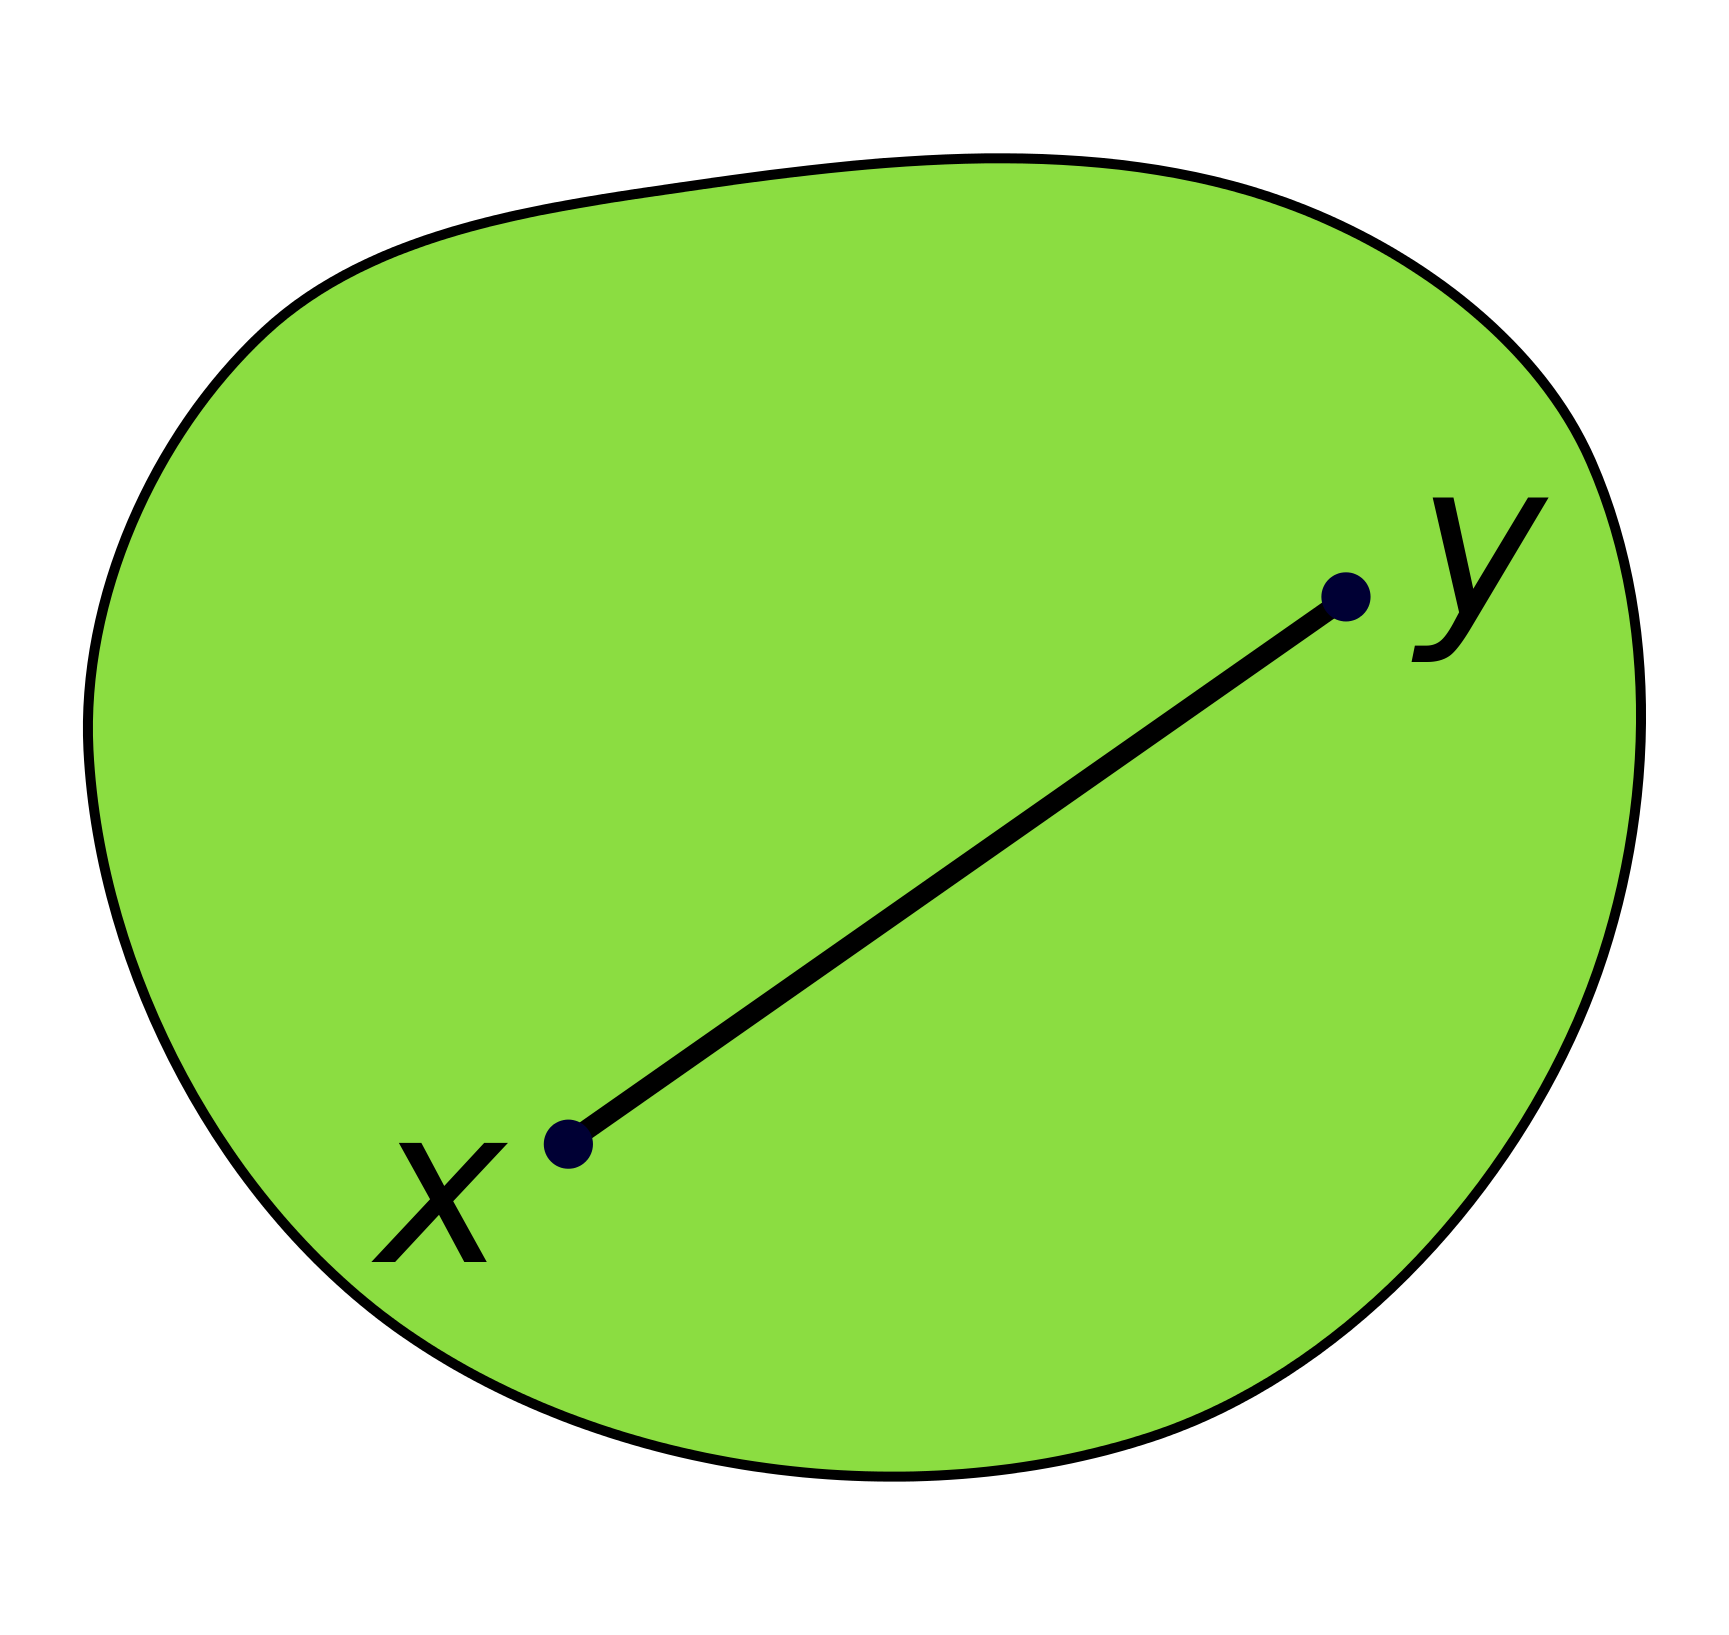
\includegraphics[width=\linewidth]{convex-set}
    \caption{A convex set}
  \end{subfigure}
  \begin{subfigure}[b]{0.45\linewidth}
    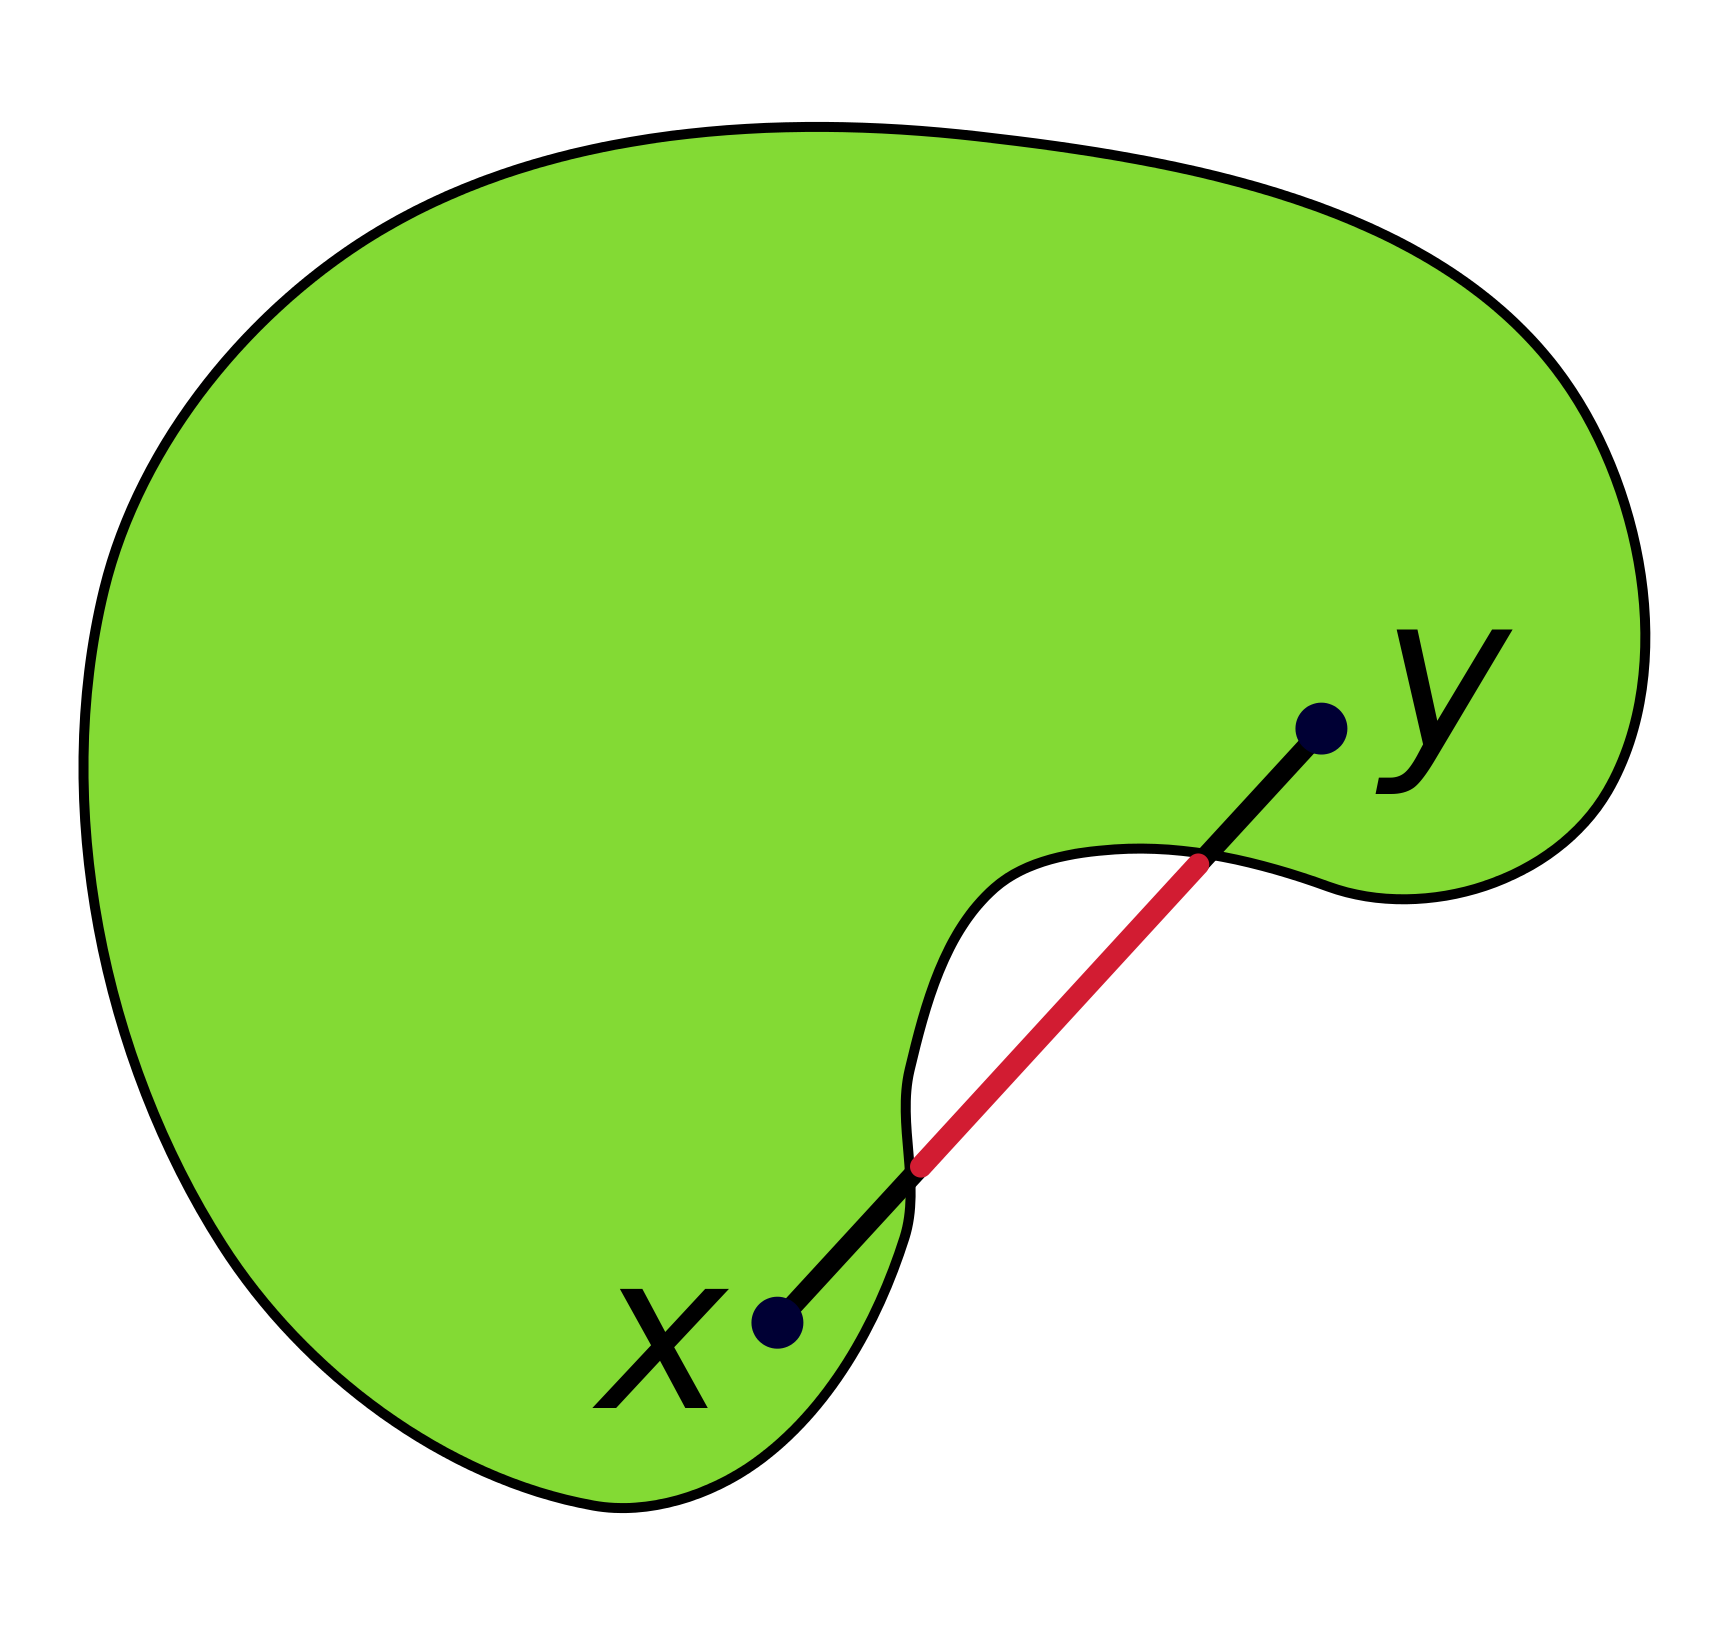
\includegraphics[width=\linewidth]{nonconvex-set}
    \caption{A non-convex set}
  \end{subfigure}
  \caption{What convex sets look like}
  \label{fig:convexset}
\end{figure}

A set $\calC \subseteq \R^d$ is \term{convex} if
\[t\x + (1-t)\y \in \calC\]
for all $\vec{x}, \vec{y} \in \calC$ and all $t \in [0,1]$.

Geometrically, this means that all the points on the line segment between any two points in $\calC$ are also in $\calC$.
See Figure \ref{fig:convexset} for a visual.

Why do we care whether or not a set is convex?
We will see later that the nature of minima can depend greatly on whether or not the feasible set is convex.
Undesirable pathological results can occur when we allow the feasible set to be arbitrary, so for proofs we will need to assume that it is convex.
Fortunately, we often want to minimize over all of $\R^d$, which is easily seen to be a convex set.

\subsubsection{Basics of convex functions}
In the remainder of this section, assume $f : \R^d \to \R$ unless otherwise noted. We'll start with the definitions and then give some results.

A function $f$ is \term{convex} if
\[f(t\vec{x} + (1-t)\vec{y}) \leq t f(\vec{x}) + (1-t)f(\vec{y})\]
for all $\vec{x}, \vec{y} \in \dom f$ and all $t \in [0,1]$.

If the inequality holds strictly (i.e. $<$ rather than $\leq$) for all $t \in (0,1)$ and $\x \neq \y$, then we say that $f$ is \term{strictly convex}.

A function $f$ is \term{strongly convex with parameter $m$} (or \term{$m$-strongly convex}) if the function
\[\x \mapsto f(\x) - \frac{m}{2}\|\x\|_2^2\]
is convex.

These conditions are given in increasing order of strength; strong convexity implies strict convexity which implies convexity.

%\begin{proposition}
%If $f$ is strictly convex, then $f$ is convex.
%\end{proposition}
%\begin{proof}
%Suppose $\x, \y \in \dom f$ and $t \in [0,1]$. We break it down by cases:
%\begin{enumerate}
%\item $\x \neq \y$ and $t \in (0,1)$: the convexity condition is a clear consequence of the strict convexity condition.
%\item $\x = \y$ and $t \in [0,1]$: we have
%\[f(t\x + (1-t)\y) = f(t\x + (1-t)\x) = f(\x) = f(\x) + t f(\x) - t f(\y) = t f(\x) + (1-t)f(\y)\]
%so the condition holds.
%\item $t = 0$: then
%\[f(t\x + (1-t)\y) = f(\y) = t f(\x) + (1-t)f(\y)\]
%\item $t = 1$: similar to the $t = 0$ case.
%\end{enumerate}
%Hence $f$ is convex.
%\end{proof}
%
%\begin{proposition}
%If $f$ is $m$-strongly convex, then $f$ is strictly convex.
%\end{proposition}
%\begin{proof}
%To-do.
%\end{proof}

\begin{figure}
  \centering
  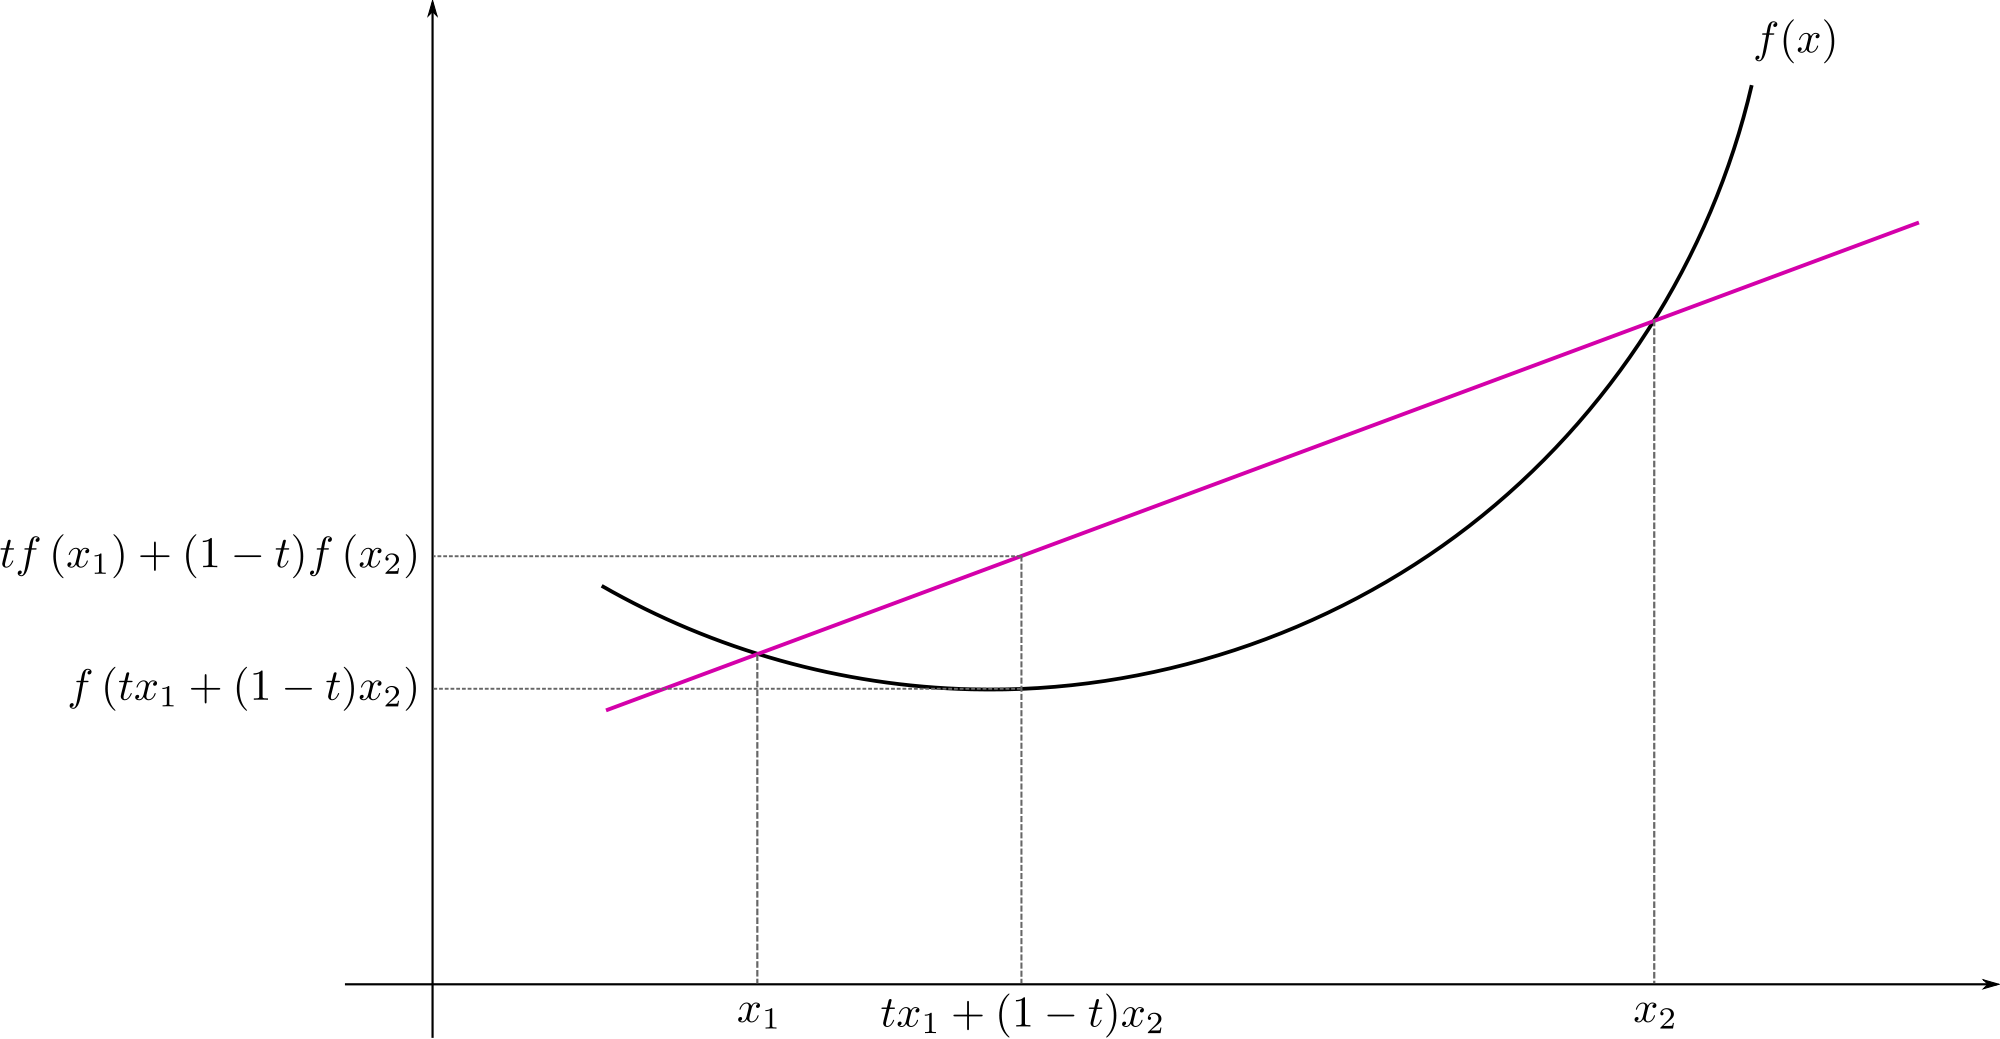
\includegraphics[width=\linewidth]{convex-function}
  \caption{What convex functions look like}
  \label{fig:convexfunction}
\end{figure}

Geometrically, convexity means that the line segment between two points on the graph of $f$ lies on or above the graph itself.
See Figure \ref{fig:convexfunction} for a visual.

Strict convexity means that the graph of $f$ lies strictly above the line segment, except at the segment endpoints.
(So actually the function in the figure appears to be strictly convex.)

\subsubsection{Consequences of convexity}
Why do we care if a function is (strictly/strongly) convex?

Basically, our various notions of convexity have implications about the nature of minima.
It should not be surprising that the stronger conditions tell us more about the minima.

\begin{proposition}
Let $\calX$ be a convex set.
If $f$ is convex, then any local minimum of $f$ in $\calX$ is also a global minimum.
\end{proposition}
\begin{proof}
Suppose $f$ is convex, and let $\x^*$ be a local minimum of $f$ in $\calX$.
Then for some neighborhood $\calN \subseteq \calX$ about $\x^*$,
\[f(\x) \geq f(\x^*) \tab \forall \x \in \calN\]
Suppose towards a contradiction that there exists $\xye \in \calX$ such that $f(\xye) < f(\x^*)$.
Consider the line segment $\x(t) = t\x^* + (1-t)\xye, ~ t \in [0,1]$, noting that $\x(t) \in \calX$ by the convexity of $\calX$.
Then by the convexity of $f$,
\[f(\x(t)) \leq tf(\x^*) + (1-t)f(\xye) < tf(\x^*) + (1-t)f(\x^*) = f(\x^*)\]
for all $t \in (0,1)$.

We can pick $t$ to be sufficiently close to $1$ that $\x(t) \in \calN$; then $f(\x(t)) \geq f(\x^*)$ by the definition of $\calN$, but $f(\x(t)) < f(\x^*)$ by the above inequality, a contradiction.

It follows that $f(\x^*) \leq f(\x)$ for all $\x \in \calX$, so $\x^*$ is a global minimum of $f$ in $\calX$.
\end{proof}

\begin{proposition}
Let $\calX$ be a convex set.
If $f$ is strictly convex, then there exists at most one local minimum of $f$ in $\calX$.
Consequently, if it exists it is the unique global minimum of $f$ in $\calX$.
\end{proposition}
\begin{proof}
The second sentence follows from the first, so all we must show is that if a local minimum exists in $\calX$ then it is unique.

Suppose $\x^*$ is a local minimum of $f$ in $\calX$, and suppose towards a contradiction that there exists a local minimum $\xye \in \calX$ such that $\xye \neq \x^*$.

Since $f$ is strictly convex, it is convex, so $\x^*$ and $\xye$ are both global minima of $f$ in $\calX$ by the previous result.
Hence $f(\x^*) = f(\xye)$.
Consider the line segment $\x(t) = t\x^* + (1-t)\xye, ~ t \in [0,1]$, which again must lie entirely in $\calX$.
By the strict convexity of $f$,
\[f(\x(t)) < tf(\x^*) + (1-t)f(\xye) = tf(\x^*) + (1-t)f(\x^*) = f(\x^*)\]
for all $t \in (0,1)$.
But this contradicts the fact that $\x^*$ is a global minimum.
Therefore if $\xye$ is a local minimum of $f$ in $\calX$, then $\xye = \x^*$, so $\x^*$ is the unique minimum in $\calX$.
\end{proof}

It is worthwhile to examine how the feasible set affects the optimization problem.
We will see why the assumption that $\calX$ is convex is needed in the results above.

Consider the function $f(x) = x^2$, which is a strictly convex function.
The unique global minimum of this function in $\R$ is $x = 0$.
But let's see what happens when we change the feasible set $\calX$.
\begin{enumerate}[(i)]
\item $\calX = \{1\}$: This set is actually convex, so we still have a unique global minimum.
But it is not the same as the unconstrained minimum!

\item $\calX = \R \setminus \{0\}$: This set is non-convex, and we can see that $f$ has no minima in $\calX$.
For any point $x \in \calX$, one can find another point $y \in \calX$ such that $f(y) < f(x)$.

\item $\calX = (-\infty,-1] \cup [0,\infty)$: This set is non-convex, and we can see that there is a local minimum ($x = -1$) which is distinct from the global minimum ($x = 0$).

\item $\calX = (-\infty,-1] \cup [1,\infty)$: This set is non-convex, and we can see that there are two global minima ($x = \pm 1$).
\end{enumerate}

\subsubsection{Showing that a function is convex}
Hopefully the previous section has convinced the reader that convexity is an important property.
Next we turn to the issue of showing that a function is (strictly/strongly) convex.
It is of course possible (in principle) to directly show that the condition in the definition holds, but this is usually not the easiest way.

\begin{proposition}
Norms are convex.
\end{proposition}
\begin{proof}
Let $\|\cdot\|$ be a norm on $\R^d$. Then for all $\x, \y \in \R^d$ and $t \in [0,1]$,
\[\|t\x + (1-t)\y\| \leq \|t\x\| + \|(1-t)\y\| = |t|\|\x\| + |1-t|\|\y\| = t\|\x\| + (1-t)\|\y\|\]
where we have used respectively the triangle inequality, the homogeneity of norms, and the fact that $t$ and $1-t$ are nonnegative.
Hence $\|\cdot\|$ is convex.
\end{proof}

\begin{proposition}
Suppose $f$ is differentiable. Then $f$ is convex if and only if
\[f(\y) \geq f(\x) + \angle{\nabla f(\x), \y - \x}\]
for all $\x, \y \in \dom f$.
\end{proposition}
\begin{proof}
To-do.
\end{proof}

\begin{proposition}
Suppose $f$ is twice differentiable.
Then
\begin{enumerate}[(i)]
\item $f$ is convex if and only if $\nabla^2 f(\x) \succeq 0$ for all $\x \in \dom f$.
\item If $\nabla^2 f(\x) \succ 0$ for all $\x \in \dom f$, then $f$ is strictly convex.
\item $f$ is $m$-strongly convex if and only if $\nabla^2 f(\x) \succeq mI$ for all $\x \in \dom f$.
\end{enumerate}
\end{proposition}
\begin{proof}
Omitted.
\end{proof}

\begin{proposition}
If $f$ is convex and $\alpha \geq 0$, then $\alpha f$ is convex.
\end{proposition}
\begin{proof}
Suppose $f$ is convex and $\alpha \geq 0$. Then for all $\x, \y \in \dom(\alpha f) = \dom f$,
\begin{align*}
(\alpha f)(t\x + (1-t)\y) &= \alpha f(t\x + (1-t)\y) \\
&\leq \alpha\left(tf(\x) + (1-t)f(\y)\right) \\
&= t(\alpha f(\x)) + (1-t)(\alpha f(\y)) \\
&= t(\alpha f)(\x) + (1-t)(\alpha f)(\y)
\end{align*}
so $\alpha f$ is convex.
\end{proof}

\begin{proposition}
If $f$ and $g$ are convex, then $f+g$ is convex.
Furthermore, if $g$ is strictly convex, then $f+g$ is strictly convex, and if $g$ is $m$-strongly convex, then $f+g$ is $m$-strongly convex.
\end{proposition}
\begin{proof}
Suppose $f$ and $g$ are convex. Then for all $\x, \y \in \dom (f+g) = \dom f \cap \dom g$,
\begin{align*}
(f+g)(t\x + (1-t)\y) &= f(t\x + (1-t)\y) + g(t\x + (1-t)\y) \\
&\leq tf(\x) + (1-t)f(\y) + g(t\x + (1-t)\y) & \text{convexity of $f$} \\
&\leq tf(\x) + (1-t)f(\y) + tg(\x) + (1-t)g(\y) & \text{convexity of $g$} \\
&= t(f(\x) + g(\x)) + (1-t)(f(\y) + g(\y)) \\
&= t(f+g)(\x) + (1-t)(f+g)(\y)
\end{align*}
so $f + g$ is convex.

If $g$ is strictly convex, the second inequality above holds strictly for $\x \neq \y$ and $t \in (0,1)$, so $f+g$ is strictly convex.

If $g$ is $m$-strongly convex, then the function $h(\x) \equiv g(\x) - \frac{m}{2}\|\x\|_2^2$ is convex, so $f+h$ is convex.
But
\[(f+h)(\x) \equiv f(\x) + h(\x) \equiv f(\x) + g(\x) - \frac{m}{2}\|\x\|_2^2 \equiv (f+g)(\x) - \frac{m}{2}\|\x\|_2^2\]
so $f+g$ is $m$-strongly convex.
\end{proof}

\begin{proposition}
If $f_1, \dots, f_n$ are convex and $\alpha_1, \dots, \alpha_n \geq 0$, then
\[\sum_{i=1}^n \alpha_i f_i\]
is convex.
\end{proposition}
\begin{proof}
Follows from the previous two propositions by induction.
\end{proof}

\begin{proposition}
If $f$ is convex, then $g(\vec{x}) \equiv f(A\x + \vec{b})$ is convex for any appropriately-sized $A$ and $\b$.
\end{proposition}
\begin{proof}
Suppose $f$ is convex and $g$ is defined like so. Then for all $\x, \y \in \dom g$,
\begin{align*}
g(t\x + (1-t)\y) &= f(A(t\x + (1-t)\y) + \b) \\
&= f(tA\x + (1-t)A\y + \b) \\
&= f(tA\x + (1-t)A\y + t\b + (1-t)\b) \\
&= f(t(A\x + \b) + (1-t)(A\y + \b)) \\
&\leq tf(A\x + \b) + (1-t)f(A\y + \b) & \text{convexity of $f$} \\
&= tg(\x) + (1-t)g(\y)
\end{align*}
Thus $g$ is convex.
\end{proof}

\begin{proposition}
If $f$ and $g$ are convex, then $h(\vec{x}) \equiv \max\{f(\vec{x}), g(\vec{x})\}$ is convex.
\end{proposition}
\begin{proof}
Suppose $f$ and $g$ are convex and $h$ is defined like so. Then for all $\x, \y \in \dom h$,
\begin{align*}
h(t\x + (1-t)\y) &= \max\{f(t\x + (1-t)\y), g(t\x + (1-t)\y)\} \\
&\leq \max\{tf(\x) + (1-t)f(\y), tg(\x) + (1-t)g(\y)\} \\
&\leq \max\{tf(\x), tg(\x)\} + \max\{(1-t)f(\y), (1-t)g(\y)\} \\
&= t\max\{f(\x), g(\x)\} + (1-t)\max\{f(\y), g(\y)\} \\
&= th(\x) + (1-t)h(\y)
\end{align*}
Note that in the first inequality we have used convexity of $f$ and $g$ plus the fact that $a \leq c, b \leq d$ implies $\max\{a,b\} \leq \max\{c,d\}$.
In the second inequality we have used the fact that $\max\{a+b, c+d\} \leq \max\{a,c\} + \max\{b,d\}$.

Thus $h$ is convex.
\end{proof}

\subsubsection{Examples}
A good way to gain intuition about the distinction between convex, strictly convex, and strongly convex functions is to consider examples where the stronger property fails to hold.

Functions that are convex but not strictly convex:
\begin{enumerate}[(i)]
\item $f(\x) = \w\tran\x + \alpha$ for any $\w \in \R^d, \alpha \in \R$.
Such a function is called an \term{affine function}, and it is both convex and concave.
(In fact, a function is affine if and only if it is both convex and concave.)
Note that linear functions and constant functions are special cases of affine functions.
\item $f(\x) = \|\x\|_1$
\end{enumerate}

Functions that are strictly but not strongly convex:
\begin{enumerate}[(i)]
\item $f(x) = x^4$.
This example is interesting because it is strictly convex but you cannot show this fact via a second-order argument (since $f''(0) = 0$).
\item $f(x) = \exp(x)$.
This example is interesting because it's bounded below but has no local minimum.
\item $f(x) = -\log x$.
This example is interesting because it's strictly convex but not bounded below.
\end{enumerate}

Functions that are strongly convex:
\begin{enumerate}[(i)]
\item $f(\x) = \|\x\|_2^2$
\end{enumerate}


\subsection{Orthogonal projections}
We now consider a particular kind of optimization problem that is particularly well-understood and can often be solved in closed form: given some point $\x$ in an inner product space $V$, find the closest point to $\x$ in a subspace $S$ of $V$.
This process is referred to as \term{projection onto a subspace}.

The following diagram should make it geometrically clear that, at least in Euclidean space, the solution is intimately related to orthogonality and the Pythagorean theorem:
\begin{center}

\includegraphics[width=0.5\linewidth]{orthogonal-projection}
\end{center}
Here $\y$ is an arbitrary element of the subspace $S$, and $\y^*$ is the point in $S$ such that $\x-\y^*$ is perpendicular to $S$.
The hypotenuse of a right triangle (in this case $\|\x-\y\|$) is always longer than either of the legs (in this case $\|\x-\y^*\|$ and $\|\y^*-\y\|$), and when $\y \neq \y^*$ there always exists such a triangle between $\x$, $\y$, and $\y^*$.

Our intuition from Euclidean space suggests that the closest point to $\x$ in $S$ has the perpendicularity property described above, and we now show that this is indeed the case.
\begin{proposition}
Suppose $\x \in V$ and $\y \in S$.
Then $\y^*$ is the unique minimizer of $\|\x-\y\|$ over $\y \in S$ if and only if $\x-\y^* \perp S$.
\end{proposition}
\begin{proof}
$(\implies)$
Suppose $\y^*$ is the unique minimizer of $\|\x-\y\|$ over $\y \in S$.
That is, $\|\x-\y^*\| \leq \|\x-\y\|$ for all $\y \in S$, with equality only if $\y = \y^*$.
Fix $\vec{v} \in S$ and observe that
\begin{align*}
g(t) &:= \|\x-\y^*+t\vec{v}\|^2 \\
&= \inner{\x-\y^*+t\vec{v}}{\x-\y^*+t\vec{v}} \\
&= \inner{\x-\y^*}{\x-\y^*} - 2t\inner{\x-\y^*}{\vec{v}} + t^2\inner{\vec{v}}{\vec{v}} \\
&= \|\x-\y^*\|^2 - 2t\inner{\x-\y^*}{\vec{v}} + t^2\|\vec{v}\|^2
\end{align*}
must have a minimum at $t = 0$ as a consequence of this assumption.
Thus
\[0 = g'(0) = \left.-2\inner{\x-\y^*}{\vec{v}} + 2t\|\vec{v}\|^2\right|_{t=0} = -2\inner{\x-\y^*}{\vec{v}}\]
giving $\x-\y^* \perp \vec{v}$.
Since $\vec{v}$ was arbitrary in $S$, we have $\x-\y^* \perp S$ as claimed.

$(\impliedby)$
Suppose $\x-\y^* \perp S$.
Observe that for any $\y \in S$, $\y^*-\y \in S$ because $\y^* \in S$ and $S$ is closed under subtraction.
Under the hypothesis, $\x-\y^* \perp \y^*-\y$, so by the Pythagorean theorem,
\[\|\x-\y\| = \|\x-\y^*+\y^*-\y\| = \|\x-\y^*\| + \|\y^*-\y\| \geq \|\x - \y^*\|\]
and in fact the inequality is strict when $\y \neq \y^*$ since this implies $\|\y^*-\y\| > 0$.
Thus $\y^*$ is the unique minimizer of $\|\x-\y\|$ over $\y \in S$.
\end{proof}
Since a unique minimizer in $S$ can be found for any $\x \in V$, we can define an operator
\[P\x = \argmin_{\y \in S} \|\x-\y\|\]
Observe that $P\y = \y$ for any $\y \in S$, since $\y$ has distance zero from itself and every other point in $S$ has positive distance from $\y$.
Thus $P(P\x) = P\x$ for any $\x$ (i.e., $P^2 = P$) because $P\x \in S$.
The identity $P^2 = P$ is actually one of the defining properties of a \term{projection}, the other being linearity.

An immediate consequence of the previous result is that $\x - P\x \perp S$ for any $\x \in V$, and conversely that $P$ is the unique operator that satisfies this property for all $\x \in V$.
For this reason, $P$ is known as an \term{orthogonal projection}.

If we choose an orthonormal basis for the target subspace $S$, it is possible to write down a more specific expression for $P$.
\begin{proposition}
If $\e_1, \dots, \e_m$ is an orthonormal basis for $S$, then
\[P\x = \sum_{i=1}^m \inner{\x}{\e_i}\e_i\]
\end{proposition}
\begin{proof}	
Let $\e_1, \dots, \e_m$ be an orthonormal basis for $S$, and suppose $\x \in V$.
Then for all $j = 1, \dots, m$,
\begin{align*}
\biginner{\x-\sum_{i=1}^m \inner{\x}{\e_i}\e_i}{\e_j} &= \inner{\x}{\e_j} - \sum_{i=1}^m \inner{\x}{\e_i}\underbrace{\inner{\e_i}{\e_j}}_{\delta_{ij}} \\
&= \inner{\x}{\e_j} - \inner{\x}{\e_j} \\
&= 0
\end{align*}
We have shown that the claimed expression, call it $\tilde{P}\x$, satisfies $\x - \tilde{P}\x \perp \e_j$ for every element $\e_j$ of the orthonormal basis for $S$.
It follows (by linearity of the inner product) that $\x - \tilde{P}\x \perp S$, so the previous result implies $P = \tilde{P}$.
\end{proof}
The fact that $P$ is a linear operator (and thus a proper projection, as earlier we showed $P^2 = P$) follows readily from this result.

%Another useful fact about the orthogonal projection operator is that the metric it induces is \term{non-expansive}, i.e. $1$-Lipschitz.
%\begin{proposition}
%For any $\x \in V$,
%\[\|P\x\| \leq \|\x\|\]
%Thus for any $\x, \xye \in V$,
%\[\|P\x - P\xye\| \leq \|\x-\xye\|\]
%\end{proposition}
%\begin{proof}
%Suppose $\x \in V$.
%Then
%\[\|P\x\|^2 = \inner{P\x}{P\x} = \inner{\x}{P^2\x} = \inner{\x}{P\x} \leq \|\x\|\|P\x\|\]
%using respectively the self-adjointness of $P$, the fact that $P^2 = P$, and the Cauchy-Schwarz inequality.
%If $\|P\x\| = 0$, the inequality holds vacuously; otherwise we can divide both sides by $\|P\x\|$ to obtain $\|P\x\| \leq \|\x\|$.
%
%The second statement follows immediately from the first by linearity of $P$.
%\end{proof}

\newpage
\section{Probability}
Probability theory provides powerful tools for modeling and dealing with uncertainty.

\subsection{Basics}
Suppose we have some sort of randomized experiment (e.g. a coin toss, die roll) that has a fixed set of possible outcomes.
This set is called the \term{sample space} and denoted $\Omega$.

We would like to define probabilities for some \term{events}, which are subsets of $\Omega$.
The set of events is denoted $\calF$.\footnote{
    $\calF$ is required to be a $\sigma$-algebra for technical reasons; see \cite{rigorousprob}.
}
The \term{complement} of the event $A$ is another event, $A\comp = \Omega \setminus A$.

Then we can define a \term{probability measure} $\P : \calF \to [0,1]$ which must satisfy
\begin{enumerate}[(i)]
\item $\pr{\Omega} = 1$
\item \term{Countable additivity}: for any countable collection of disjoint sets $\{A_i\} \subseteq \calF$,
\[\prbigg{\bigcup_i A_i} = \sum_i \pr{A_i}\]
\end{enumerate}
The triple $(\Omega, \calF, \P)$ is called a \term{probability space}.\footnote{
    Note that a probability space is simply a measure space in which the measure of the whole space equals 1.
}

If $\pr{A} = 1$, we say that $A$ occurs \term{almost surely} (often abbreviated a.s.).\footnote{
    This is a probabilist's version of the measure-theoretic term \textit{almost everywhere}.
}, and conversely $A$ occurs \term{almost never} if $\pr{A} = 0$.

From these axioms, a number of useful rules can be derived.
\begin{proposition}
Let $A$ be an event. Then
\begin{enumerate}[(i)]
\item $\pr{A\comp} = 1 - \pr{A}$.
\item If $B$ is an event and $B \subseteq A$, then $\pr{B} \leq \pr{A}$.
\item $0 = \pr{\varnothing} \leq \pr{A} \leq \pr{\Omega} = 1$
\end{enumerate}
\end{proposition}
\begin{proof}
(i) Using the countable additivity of $\P$, we have
\[\pr{A} + \pr{A\comp} = \pr{A \dotcup A\comp} = \pr{\Omega} = 1\]

To show (ii), suppose $B \in \calF$ and $B \subseteq A$. Then
\[\pr{A} = \pr{B \dotcup (A \setminus B)} = \pr{B} + \pr{A \setminus B} \geq \pr{B}\]
as claimed.

For (iii): the middle inequality follows from (ii) since $\varnothing \subseteq A \subseteq \Omega$.
We also have
\[\pr{\varnothing} = \pr{\varnothing \dotcup \varnothing} = \pr{\varnothing} + \pr{\varnothing}\]
by countable additivity, which shows $\pr{\varnothing} = 0$.
\end{proof}

\begin{proposition}
If $A$ and $B$ are events, then $\pr{A \cup B} = \pr{A} + \pr{B} - \pr{A \cap B}$.
\end{proposition}
\begin{proof}
The key is to break the events up into their various overlapping and non-overlapping parts.
\begin{align*}
\pr{A \cup B} &= \pr{(A \cap B) \dotcup (A \setminus B) \dotcup (B \setminus A)} \\
&= \pr{A \cap B} + \pr{A \setminus B} + \pr{B \setminus A} \\
&= \pr{A \cap B} + \pr{A} - \pr{A \cap B} + \pr{B} - \pr{A \cap B} \\
&= \pr{A} + \pr{B} - \pr{A \cap B}
\end{align*}
\end{proof}

\begin{proposition}
If $\{A_i\} \subseteq \calF$ is a countable set of events, disjoint or not, then
\[\prbigg{\bigcup_i A_i} \leq \sum_i \pr{A_i}\]
\end{proposition}
This inequality is sometimes referred to as \term{Boole's inequality} or the \term{union bound}.
\begin{proof}
Define $B_1 = A_1$ and $B_i = A_i \setminus (\bigcup_{j < i} A_j)$ for $i > 1$, noting that $\bigcup_{j \leq i} B_j = \bigcup_{j \leq i} A_j$ for all $i$ and the $B_i$ are disjoint.
Then
\[\prbigg{\bigcup_i A_i} = \prbigg{\bigcup_i B_i} = \sum_i \pr{B_i} \leq \sum_i \pr{A_i}\]
where the last inequality follows by monotonicity since $B_i \subseteq A_i$ for all $i$.
\end{proof}

\subsubsection{Conditional probability}
The \term{conditional probability} of event $A$ given that event $B$ has occurred is written $\pr{A \given B}$ and defined as
\[\pr{A \given B} = \frac{\pr{A \cap B}}{\pr{B}}\]
assuming $\pr{B} > 0$.\footnote{
    In some cases it is possible to define conditional probability on events of probability zero, but this is significantly more technical so we omit it.
}

\subsubsection{Chain rule}
Another very useful tool, the \term{chain rule}, follows immediately from this definition:
\[\pr{A \cap B} = \pr{A \given B}\pr{B} = \pr{B \given A}\pr{A}\]

\subsubsection{Bayes' rule}
Taking the equality from above one step further, we arrive at the simple but crucial \term{Bayes' rule}:
\[\pr{A \given B} = \frac{\pr{B \given A}\pr{A}}{\pr{B}}\]
It is sometimes beneficial to omit the normalizing constant and write
\[\pr{A \given B} \propto \pr{A}\pr{B \given A}\]
Under this formulation, $\pr{A}$ is often referred to as the \term{prior}, $\pr{A \given B}$ as the \term{posterior}, and $\pr{B \given A}$ as the \term{likelihood}.

In the context of machine learning, we can use Bayes' rule to update our ``beliefs'' (e.g. values of our model parameters) given some data that we've observed.

\subsection{Random variables}
A \term{random variable} is some uncertain quantity with an associated probability distribution over the values it can assume.

Formally, a random variable on a probability space $(\Omega, \calF, \P)$ is a function\footnote{
    The function must be measurable.
} $X: \Omega \to \R$.\footnote{
    More generally, the codomain can be any measurable space, but $\R$ is the most common case by far and sufficient for our purposes.
}

We denote the range of $X$ by $X(\Omega) = \{X(\omega) : \omega \in \Omega\}$.
To give a concrete example (taken from \cite{pitman}), suppose $X$ is the number of heads in two tosses of a fair coin.
The sample space is
\[\Omega = \{hh, tt, ht, th\}\]
and $X$ is determined completely by the outcome $\omega$, i.e. $X = X(\omega)$.
For example, the event $X = 1$ is the set of outcomes $\{ht, th\}$.

It is common to talk about the values of a random variable without directly referencing its sample space.
The two are related by the following definition: the event that the value of $X$ lies in some set $S \subseteq \R$ is
\[X \in S = \{\omega \in \Omega : X(\omega) \in S\}\]
Note that special cases of this definition include $X$ being equal to, less than, or greater than some specified value.
For example
\[\pr{X = x} = \pr{\{\omega \in \Omega : X(\omega) = x\}}\]

A word on notation: we write $p(X)$ to denote the entire probability distribution of $X$ and $p(x)$ for the evaluation of the function $p$ at a particular value $x \in X(\Omega)$.
Hopefully this (reasonably standard) abuse of notation is not too distracting.
If $p$ is parameterized by some parameters $\theta$, we write $p(X; \vec{\theta})$ or $p(x; \vec{\theta})$, unless we are in a Bayesian setting where the parameters are considered a random variable, in which case we condition on the parameters.

\subsubsection{The cumulative distribution function}
The \term{cumulative distribution function} (c.d.f.) gives the probability that a random variable is at most a certain value:
\[F(x) = \pr{X \leq x}\]
The c.d.f. can be used to give the probability that a variable lies within a certain range:
\[\pr{a < X \leq b} = F(b) - F(a)\]

\subsubsection{Discrete random variables}
A \term{discrete random variable} is a random variable that has a countable range and assumes each value in this range with positive probability.
Discrete random variables are completely specified by their \term{probability mass function} (p.m.f.) $p : X(\Omega) \to [0,1]$ which satisfies
\[\sum_{x \in X(\Omega)} p(x) = 1\]
For a discrete $X$, the probability of a particular value is given exactly by its p.m.f.:
\[\pr{X = x} = p(x)\]

\subsubsection{Continuous random variables}
A \term{continuous random variable} is a random variable that has an uncountable range and assumes each value in this range with probability zero.
Most of the continuous random variables that one would encounter in practice are \term{absolutely continuous random variables}\footnote{
    Random variables that are continuous but not absolutely continuous are called \term{singular random variables}.
    We will not discuss them, assuming rather that all continuous random variables admit a density function.
}, which means that there exists a function $p : \R \to [0,\infty)$ that satisfies
\[F(x) \equiv \int_{-\infty}^x p(z)\dd{z}\]
The function $p$ is called a \term{probability density function} (abbreviated p.d.f.) and must satisfy
\[\int_{-\infty}^\infty p(x)\dd{x} = 1\]
The values of this function are not themselves probabilities, since they could exceed 1.
However, they do have a couple of reasonable interpretations.
One is as relative probabilities; even though the probability of each particular value being picked is technically zero, some points are still in a sense more likely than others.

One can also think of the density as determining the probability that the variable will lie in a small range about a given value.
This is because, for small $\epsilon > 0$,
\[\pr{x-\epsilon \leq X \leq x+\epsilon} = \int_{x-\epsilon}^{x+\epsilon} p(z)\dd{z} \approx 2\epsilon p(x)\]
using a midpoint approximation to the integral.

Here are some useful identities that follow from the definitions above:
\begin{align*}
\pr{a \leq X \leq b} &= \int_a^b p(x)\dd{x} \\
p(x) &= F'(x)
\end{align*}

\subsubsection{Other kinds of random variables}
There are random variables that are neither discrete nor continuous.
For example, consider a random variable determined as follows:
flip a fair coin, then the value is zero if it comes up heads, otherwise draw a number uniformly at random from $[1,2]$.
Such a random variable can take on uncountably many values, but only finitely many of these with positive probability.
We will not discuss such random variables because they are rather pathological and require measure theory to analyze.

\subsection{Joint distributions}
Often we have several random variables and we would like to get a distribution over some combination of them.
A \term{joint distribution} is exactly this.
For some random variables $X_1, \dots, X_n$, the joint distribution is written $p(X_1, \dots, X_n)$ and gives probabilities over entire assignments to all the $X_i$ simultaneously.

\subsubsection{Independence of random variables}
We say that two variables $X$ and $Y$ are \term{independent} if their joint distribution factors into their respective distributions, i.e.
\[p(X, Y) = p(X)p(Y)\]
We can also define independence for more than two random variables, although it is more complicated.
Let $\{X_i\}_{i \in I}$ be a collection of random variables indexed by $I$, which may be infinite.
Then $\{X_i\}$ are independent if for every finite subset of indices $i_1, \dots, i_k \in I$ we have
\[p(X_{i_1}, \dots, X_{i_k}) = \prod_{j=1}^k p(X_{i_j})\]
For example, in the case of three random variables, $X, Y, Z$, we require that $p(X,Y,Z) = p(X)p(Y)p(Z)$ as well as $p(X,Y) = p(X)p(Y)$, $p(X,Z) = p(X)p(Z)$, and $p(Y,Z) = p(Y)p(Z)$.

It is often convenient (though perhaps questionable) to assume that a bunch of random variables are \term{independent and identically distributed} (i.i.d.) so that their joint distribution can be factored entirely:
\[p(X_1, \dots, X_n) = \prod_{i=1}^n p(X_i)\]
where $X_1, \dots, X_n$ all share the same p.m.f./p.d.f.

\subsubsection{Marginal distributions}
If we have a joint distribution over some set of random variables, it is possible to obtain a distribution for a subset of them by ``summing out'' (or ``integrating out'' in the continuous case) the variables we don't care about:
\[p(X) = \sum_{y} p(X, y)\]

\subsection{Great Expectations}
If we have some random variable $X$, we might be interested in knowing what is the ``average'' value of $X$.
This concept is captured by the \term{expected value} (or \term{mean}) $\ev{X}$, which is defined as
\[\ev{X} = \sum_{x \in X(\Omega)} xp(x)\]
for discrete $X$ and as
\[\ev{X} = \int_{-\infty}^\infty xp(x)\dd{x}\]
for continuous $X$.

In words, we are taking a weighted sum of the values that $X$ can take on, where the weights are the probabilities of those respective values.
The expected value has a physical interpretation as the ``center of mass'' of the distribution.

\subsubsection{Properties of expected value}
A very useful property of expectation is that of linearity:
\[\bigev{\sum_{i=1}^n \alpha_i X_i + \beta} = \sum_{i=1}^n \alpha_i \ev{X_i} + \beta\]
Note that this holds even if the $X_i$ are not independent!

But if they are independent, the product rule also holds:
\[\bigev{\prod_{i=1}^n X_i} = \prod_{i=1}^n \ev{X_i}\]

\subsection{Variance}
Expectation provides a measure of the ``center'' of a distribution, but frequently we are also interested in what the ``spread'' is about that center.
We define the variance $\var{X}$ of a random variable $X$ by
\[\var{X} = \bigev{\left(X - \ev{X}\right)^2}\]
In words, this is the average squared deviation of the values of $X$ from the mean of $X$.
Using a little algebra and the linearity of expectation, it is straightforward to show that
\[\var{X} = \ev{X^2} - \ev{X}^2\]

\subsubsection{Properties of variance}
Variance is not linear (because of the squaring in the definition), but one can show the following:
\[\var{\alpha X + \beta} = \alpha^2 \var{X}\]
Basically, multiplicative constants become squared when they are pulled out, and additive constants disappear (since the variance contributed by a constant is zero).

Furthermore, if $X_1, \dots, X_n$ are uncorrelated\footnote{
    We haven't defined this yet; see the Correlation section below
}, then
\[\var{X_1 + \dots + X_n} = \var{X_1} + \dots + \var{X_n}\]

\subsubsection{Standard deviation}
Variance is a useful notion, but it suffers from that fact the units of variance are not the same as the units of the random variable (again because of the squaring).
To overcome this problem we can use \term{standard deviation}, which is defined as $\sqrt{\var{X}}$.
The standard deviation of $X$ has the same units as $X$.

\subsection{Covariance}
Covariance is a measure of the linear relationship between two random variables.
We denote the covariance between $X$ and $Y$ as $\cov{X}{Y}$, and it is defined to be
\[\cov{X}{Y} = \ev{(X-\ev{X})(Y-\ev{Y})}\]
Note that the outer expectation must be taken over the joint distribution of $X$ and $Y$.

Again, the linearity of expectation allows us to rewrite this as
\[\cov{X}{Y} = \ev{XY} - \ev{X}\ev{Y}\]
Comparing these formulas to the ones for variance, it is not hard to see that $\var{X} = \cov{X}{X}$.

A useful property of covariance is that of \term{bilinearity}:
\begin{align*}
\cov{\alpha X + \beta Y}{Z} &= \alpha\cov{X}{Z} + \beta\cov{Y}{Z} \\
\cov{X}{\alpha Y + \beta Z} &= \alpha\cov{X}{Y} + \beta\cov{X}{Z}
\end{align*}

\subsubsection{Correlation}
Normalizing the covariance gives the \term{correlation}:
\[\rho(X, Y) = \frac{\cov{X}{Y}}{\sqrt{\var{X}\var{Y}}}\]
Correlation also measures the linear relationship between two variables, but unlike covariance always lies between $-1$ and $1$.

Two variables are said to be \term{uncorrelated} if $\cov{X}{Y} = 0$ because $\cov{X}{Y} = 0$ implies that $\rho(X, Y) = 0$.
If two variables are independent, then they are uncorrelated, but the converse does not hold in general.

\subsection{Random vectors}
So far we have been talking about \term{univariate distributions}, that is, distributions of single variables.
But we can also talk about \term{multivariate distributions} which give distributions of \term{random vectors}:
\[\bX = \matlit{X_1 \\ \vdots \\ X_n}\]
The summarizing quantities we have discussed for single variables have natural generalizations to the multivariate case.

Expectation of a random vector is simply the expectation applied to each component:
\[\ev{\bX} = \matlit{\ev{X_1} \\ \vdots \\ \ev{X_n}}\]

The variance is generalized by the \term{covariance matrix}:
\[\mat{\Sigma} = \ev{(\bX - \ev{\bX})(\bX - \ev{\bX})\tran} = \matlit{
\var{X_1} & \cov{X_1}{X_2} & \hdots & \cov{X_1}{X_n} \\
\cov{X_2}{X_1} & \var{X_2} & \hdots & \cov{X_2}{X_n} \\
\vdots & \vdots & \ddots & \vdots \\
\cov{X_n}{X_1} & \cov{X_n}{X_2} & \hdots & \var{X_n}
}\]
That is, $\Sigma_{ij} = \cov{X_i}{X_j}$.
Since covariance is symmetric in its arguments, the covariance matrix is also symmetric.
It's also positive semi-definite: for any $\x$,
\[\x\tran\mat{\Sigma}\x = \x\tran\ev{(\bX - \ev{\bX})(\bX - \ev{\bX})\tran}\x = \ev{\x\tran(\bX - \ev{\bX})(\bX - \ev{\bX})\tran\x} = \ev{((\bX - \ev{\bX})\tran\x)^2} \geq 0\]
The inverse of the covariance matrix, $\mat{\Sigma}\inv$, is sometimes called the \term{precision matrix}.

\subsection{Estimation of Parameters}
Now we get into some basic topics from statistics.
We make some assumptions about our problem by prescribing a \term{parametric} model (e.g. a distribution that describes how the data were generated), then we fit the parameters of the model to the data.
How do we choose the values of the parameters?

\subsubsection{Maximum likelihood estimation}
A common way to fit parameters is \term{maximum likelihood estimation} (MLE).
The basic principle of MLE is to choose values that ``explain'' the data best by maximizing the probability/density of the data we've seen as a function of the parameters.
Suppose we have random variables $X_1, \dots, X_n$ and corresponding observations $x_1, \dots, x_n$.
Then
\[\hat{\vec{\theta}}_\textsc{mle} = \argmax_\vec{\theta} \calL(\vec{\theta})\]
where $\calL$ is the \term{likelihood function}
\[\calL(\vec{\theta}) = p(x_1, \dots, x_n; \vec{\theta})\]
Often, we assume that $X_1, \dots, X_n$ are i.i.d. Then we can write
\[p(x_1, \dots, x_n; \theta) = \prod_{i=1}^n p(x_i; \vec{\theta})\]
At this point, it is usually convenient to take logs, giving rise to the \term{log-likelihood}
\[\log\calL(\vec{\theta}) = \sum_{i=1}^n \log p(x_i; \vec{\theta})\]
This is a valid operation because the probabilities/densities are assumed to be positive, and since log is a monotonically increasing function, it preserves ordering.
In other words, any maximizer of $\log\calL$ will also maximize $\calL$.

For some distributions, it is possible to analytically solve for the maximum likelihood estimator.
If $\log\calL$ is differentiable, setting the derivatives to zero and trying to solve for $\vec{\theta}$ is a good place to start.

\subsubsection{Maximum a posteriori estimation}
A more Bayesian way to fit parameters is through \term{maximum a posteriori estimation} (MAP).
In this technique we assume that the parameters are a random variable, and we specify a prior distribution $p(\vec{\theta})$.
Then we can employ Bayes' rule to compute the posterior distribution of the parameters given the observed data:
\[p(\vec{\theta} \given x_1, \dots, x_n) \propto p(\vec{\theta})p(x_1, \dots, x_n \given \vec{\theta})\]
Computing the normalizing constant is often intractable, because it involves integrating over the parameter space, which may be very high-dimensional.
Fortunately, if we just want the MAP estimate, we don't care about the normalizing constant!
It does not affect which values of $\vec{\theta}$ maximize the posterior.
So we have
\[\hat{\vec{\theta}}_\textsc{map} = \argmax_\vec{\theta} p(\vec{\theta})p(x_1, \dots, x_n \given \vec{\theta})\]
Again, if we assume the observations are i.i.d., then we can express this in the equivalent, and possibly friendlier, form
\[\hat{\vec{\theta}}_\textsc{map} = \argmax_\vec{\theta} \left(\log p(\vec{\theta}) + \sum_{i=1}^n \log p(x_i \given \vec{\theta})\right)\]
A particularly nice case is when the prior is chosen carefully such that the posterior comes from the same family as the prior.
In this case the prior is called a \term{conjugate prior}.
For example, if the likelihood is binomial and the prior is beta, the posterior is also beta.
There are many conjugate priors; the reader may find this \href{https://en.wikipedia.org/wiki/Conjugate_prior#Table_of_conjugate_distributions}{table of conjugate priors} useful.

\subsection{The Gaussian distribution}
There are many distributions, but one of particular importance is the \term{Gaussian distribution}, also known as the \term{normal distribution}.
It is a continuous distribution, parameterized by its mean $\bm\mu \in \R^d$ and positive-definite covariance matrix $\mat{\Sigma} \in \R^{d \times d}$, with density
\[p(\x; \bm\mu, \mat{\Sigma}) = \frac{1}{\sqrt{(2\pi)^d \det(\mat{\Sigma})}}\exp\left(-\frac{1}{2}(\x - \bm\mu)\tran\mat{\Sigma}\inv(\x - \bm\mu)\right)\]
Note that in the special case $d = 1$, the density is written in the more recognizable form
\[p(x; \mu, \sigma^2) = \frac{1}{\sqrt{2\pi\sigma^2}}\exp\left(-\frac{(x-\mu)^2}{2\sigma^2}\right)\]
We write $\vec{X} \sim \calN(\bm\mu, \mat{\Sigma})$ to denote that $\vec{X}$ is normally distributed with mean $\bm\mu$ and variance $\mat{\Sigma}$.

\subsubsection{The geometry of multivariate Gaussians}
The geometry of the multivariate Gaussian density is intimately related to the geometry of positive definite quadratic forms, so make sure the material in that section is well-understood before tackling this section.

First observe that the p.d.f. of the multivariate Gaussian can be rewritten as
\[p(\x; \bm\mu, \mat{\Sigma}) = g(\xye\tran\mat{\Sigma}\inv\xye)\]
where $\xye = \x - \bm\mu$ and $g(z) = [(2\pi)^d \det(\mat{\Sigma})]^{-\frac{1}{2}}\exp\left(-\frac{z}{2}\right)$.
Writing the density in this way, we see that after shifting by the mean $\bm\mu$, the density is really just a simple function of its precision matrix's quadratic form.

Here is a key observation: this function $g$ is \term{strictly monotonically decreasing} in its argument.
That is, $g(a) > g(b)$ whenever $a < b$.
Therefore, small values of $\xye\tran\mat{\Sigma}\inv\xye$ (which generally correspond to points where $\xye$ is closer to $\vec{0}$, i.e. $\x \approx \bm\mu$) have relatively high probability densities, and vice-versa.
Furthermore, because $g$ is \textit{strictly} monotonic, it is injective, so the $c$-isocontours of $p(\x; \bm\mu, \mat{\Sigma})$ are the $g\inv(c)$-isocontours of the function $\x \mapsto \xye\tran\mat{\Sigma}\inv\xye$.
That is, for any $c$,
\[\{\x \in \R^d : p(\x; \bm\mu, \mat{\Sigma}) = c\} = \{\x \in \R^d : \xye\tran\mat{\Sigma}\inv\xye = g\inv(c)\}\]
In words, these functions have the same isocontours but different isovalues.

Recall the executive summary of the geometry of positive definite quadratic forms: the isocontours of $f(\x) = \x\tran\A\x$ are ellipsoids such that the axes point in the directions of the eigenvectors of $\A$, and the lengths of these axes are proportional to the inverse square roots of the corresponding eigenvalues.
Therefore in this case, the isocontours of the density are ellipsoids (centered at $\bm\mu$) with axis lengths proportional to the inverse square roots of the eigenvalues of $\mat{\Sigma}\inv$, or equivalently, the square roots of the eigenvalues of $\mat{\Sigma}$.


\newpage
\section*{Acknowledgements}
The author would like to thank Michael Franco for suggested clarifications.

\bibliography{math4ml}
\addcontentsline{toc}{section}{References}
\bibliographystyle{ieeetr}
\nocite{*}
\end{document}
